\documentclass[12pt]{article}

% \usepackage{identfirst}

\usepackage[utf8]{inputenc}
\usepackage[T2A]{fontenc}
\usepackage[russian]{babel}

\usepackage{csquotes}
\usepackage{amsmath}

\usepackage{makecell}
\usepackage{tabularx}
\usepackage{float}
\usepackage[toc]{appendix}

% \usepackage{listings}
\usepackage[newfloat]{minted}

\usepackage[
backend=biber,
style=gost-numeric,
sorting=none
]{biblatex}


\usepackage[a4paper,top=20mm,bottom=20mm,left=30mm,right=10mm]{geometry}

\usepackage{tocloft}
\usepackage{caption}
\usepackage{subcaption}

\usepackage{mathtools}

% \usepackage{tikz}
\usepackage{pgf-umlcd}
\usepackage{tikzit}

\usepackage{pifont}
\usepackage{flowchart}

\renewcommand{\umlfillcolor}{white}
\renewcommand{\umldrawcolor}{black}
% \usepackage{underscore}

\renewcommand{\cftsecleader}{\cftdotfill{\cftdotsep}}

% \newenvironment{code}{\captionsetup{type=listing}}{}
\SetupFloatingEnvironment{listing}{name=Листинг}

\newcommand{\intro}[1]{
    \stepcounter{section}
    \section*{\hfillПРИЛОЖЕНИЕ \arabic{section}}
    \begin{center}
        \bf{#1}
    \end{center}
    \markboth{\MakeUppercase{#1}}{}
    \addcontentsline{toc}{section}{Приложение \arabic{section}. #1}
}

\usepackage{titlesec}

\setcounter{secnumdepth}{4}

\titleformat{\paragraph}
{\normalfont\normalsize\bfseries}{\theparagraph}{1em}{}
\titlespacing*{\paragraph}
{0pt}{3.25ex plus 1ex minus .2ex}{1.5ex plus .2ex}

\addbibresource{references.bib}

\input{block-schemas.tikzstyles}

\author{Савицкий Илья Павлович}
\title{Жадные алгоритмы для построения многопроцессорного списочного расписания}
\date{Москва, 2022}

% \pgfsetlayers{connectionlayers}

\begin{document}
\makeatletter
\begin{titlepage}
    \begin{center}
        
\includegraphics[width=9cm]{imgs/msulogo.png}\\
        \small
        \centerline{Московский государственный университет имени М.В. Ломоносова}
        \centerline{Факультет вычислительной математики и кибернетики}
        \centerline{Кафедра автоматизации систем вычислительных комплексов}
        \centerline{}
        \Large
        \vfill
        {\@author}\\
        \null
        {\LARGE \bf
        \@title
        }\\
        \null \null
        {\large Выпускная квалификационная работа}\\
        \null \null
    \end{center}
    \begin{flushright}
        {\bf Научный руководитель:}\\
        Доцент, к.т.н \\Костенко Валерий Алексеевич\\
        ~\\
        % {\bf Научный консультант:}\\
        % к.ф.-м.н.\\Иванов Иван Иванович\\
        \vfill
    \end{flushright}
    \centerline{Москва, 2023}
\end{titlepage}
\setcounter{page}{2}

\newpage
\begin{abstract}
    Построение многопроцессорного расписания это NP-трудная задача. Точный полиномиальный алгоритм для решения этой задачи неизвестен. В данной работе приводятся два возможных варианта решения задачи с дополнительным ограничением на количество передач при помощи жадных алгоритмов.
\end{abstract}
\newpage
\tableofcontents
% ----------------------------------------------------------------------------------------------------------------------
\newpage
\section{Введение}
Классическая задача построения расписания хорошо изучена и досканально описана в \cite{Coffman}. Поскольку данная задача принадлежит к классу NP-трудных, не существует алгоритма, который за полиномиальное время даст точный ответ, но существуют алгоритмы, которые дают приближенные результаты. Большинство таких алгоритмов резделяются на две категории: \textit{конструктивные} и \textit{итерационные}. Из основных примеров можно выделить (большинство из них упомянуты в \cite{Kostenko_2017}):
\begin{itemize}
    \item Конструктивные алгоритмы
    \begin{enumerate}
        \item Алгоритмы, основанные на поиске максимального потока в сети
        \item Алгоритмы, основанные на методах динамического программирования
        \item Алгоитмы, основанные на методе ветвей и границ
        \item Жадные алгоритмы
        \item Жадные алгоритмы с процедурой ограниченного перебора
    \end{enumerate}
    \item Итерационные алгоритмы
    \begin{enumerate}
        \item Генетические алгоритмы
        \item Дифференциальная эволюция
        \item Алгоритм имитации отжига
        \item Алгоритм муравьиных колоний
    \end{enumerate}
\end{itemize}
\par
Конструктивные алгоритмы работают, строя и дополняя частичные расписания до тех пор, пока все работы не будут размещены. Итерационные же алгоритмы строят приближения расписания и оптимизируют их.
\par
В данной работе рассматриваются жадные алгоритмы с процедурой ограниченного перебора. Особенностью таких алгоритмов является баланс между двумя процессами построения расписания. Жадные стратегии строят расписание быстро, однако очень быстро могут зайти в тупик при построении расписания. В таком случае, если расписание строится си сильным отклонением от оптимального, процедура ограниченного перебора корректирует его.
% ----------------------------------------------------------------------------------------------------------------------
\newpage
\section{Цели и задачи этой работы}
Целью этой курсовой работы является разработка алгоритмов построения многопроцессорного расписания с дополнительными ограничениями на основе жадных алгоритмов.

Для достижения указанной цели требуется:
\begin{enumerate}
    \item Провести обзор алгоритмов построения списочных расписаний с целью выявления жадных критериев и схем ограниченного перебора которые могут быть модифицированы для решения данной задачи.
    \item Разработать алгоритмы.
    \item Реализовать алгоритмы.
    \item Провести исследование свойств алгоритма.
\end{enumerate}
% ----------------------------------------------------------------------------------------------------------------------
\newpage
\section{Постановка задачи}
В задаче построения расписания заданы:
\begin{enumerate}
    \item Граф потока управления $G$ без циклов, в котором дуги - зависимости по данным, а вершины - задания. Вершин $n$, дуг $m$
    \item Вычислительная система, состоящая из $p$ процессоров.
    \item Матрица $C_{n \times p}$ времени выполнения работ на процессорах. Каждая строка этой матрицы - длины выполнения $n$-й задачи на $p$ процессорах.
          % \item Матрица $D_{kl}$ передач данных между процессорами, $k=1 \dots p, l = 1 \dots p, D_{kk} = 0$. $D_{ij}$-й элемент этой матрицы - время передачи данных между процессорами $i$ и $j$.
    \item Время $d$, затрачиваемое на межпроцессорную передачу.
\end{enumerate}

Расписание определено, если заданы:
\begin{enumerate}
    \item Множества процессоров и работ
    \item Привязка - всюду определенная на множестве работ функция, которая задает распределение работ по процессорам
    \item Порядок - заданные ограничения на последовательность выполнения работ и являющиеся отношением частичного порядка, удовлетворяющее условиям ацикличности и транзитивности. Отношение порядка на множестве работ, распределенных на один процессор, является отношением полного порядка.
\end{enumerate}

\begin{figure}[!htbp]
    \ctikzfig{schedule-graph}
    \caption{Граф $G$ потока данных}
    \label{fig:DFG}
\end{figure}
Пусть дан следующий граф потока данных, изображенный на рисунке \ref{fig:DFG}.

Пусть в оптимальном расписании работы $3$ и $9$ будут поставлены на процессор $Pr1$. $2$, $5$, $8$ - на $Pr2$, а $1$, $10$, $4$ и $6$ - на $Pr3$. Рассмотрим как такое расписание будет выглядеть в различных представлениях:
\begin{enumerate}
    \item Графическое представление.

          \begin{figure}[!htbp]
              \ctikzfig{schedule-graphical-form}
              \caption{Графическое представление расписания}
              \label{fig:graphical-form}
          \end{figure}
          В такой форме представления расписания, изображенной на рисунке 2, каждой задаче сопоставляется пара из номера процессора и порядкового номера работы на процессоре, а так же секущие дуги, если задачи зависят друг от друга.
    \item Временная диаграмма.

          \begin{figure}[!htbp]
              \ctikzfig{schedule-time-diagram-new}
              \caption{Представление расписания в виде временной диаграммы}
              \label{fig:time-diagram}
          \end{figure}

          % \begin{figure}[!htbp]
          %     \ctikzfig{schedule-time-diagram}
          % \end{figure}

          В такой форме представления, показанной на рисунке \ref{fig:time-diagram}, расписания каждой задаче сопоставляется пара из номера процессора и времени старта задачи на процессоре.
\end{enumerate}
Доказано, что эти представления полностью эквивалентны и, имея одно, возможно построить другое. В предложенном решении расписание строится в виде временной диаграммы. Стоит отметить, что во временной диаграмме иогут возникать простои в расписании, как, например, на рисунке \ref{fig:time-diagram} в системе с длиной межпроцессорной передачи $d=1$, между работами $T_3$ и $T_9$ на процессоре $Pr1$, поскольку работа $T_9$ зависит от работы $T_5$, которая размещена на другой процессор.

Из входных данных задачи требуется построить расписание $HP$, то есть для $i$-й работы определить время начала ее выполнения $s_i$ и процессор $p_i$ на котором она будет выполняться, минимизировать время выполнения расписания, выполнив дополнительные ограничения.


Ограничения на корректность расписания следующие:
\begin{enumerate}
    \item Каждый процессор может одновременно выполнять не больше одной работы;
    \item Прерывание работ недопустимо, перенос частично выполненной работы на другой процессор недопустим;
    \item Если между двумя работами есть зависимость на данным, то между завершением работы-отправителя и стартом работы-получателя должен быть интервал времени, не меньший, чем задержка на передачу данных между ними (с учетом привязки работ к процессорам и маршрута передачи данных).
\end{enumerate}
\subsection{Различные постановки задачи} \label{sec:crit}
\begin{enumerate}
    \item Задача без дополнительных ограничений на расписание. Далее эта постановка будет упоминаться как \textbf{постановка $NO$}
    \item Задача с дополнительным ограничением на количество передач:
          \begin{itemize}
              \item $CR = \frac{m_{ip}}{m} < 0.4$, где $m_{ip}$ - количество передач данных между работами на каждый процессор. Далее эта постановка будет упоминаться как \textbf{постановка $CR$}
          \end{itemize}
\end{enumerate}
% ----------------------------------------------------------------------------------------------------------------------
\newpage
\section{Обзор предметной области}
% Обзоры других алгоритмов приведены в \cite{Shakhbazyan_1981,Davis_2011}
\subsection{Критерии обзора}
Ниже приведены критерии, по которым будут рассматриваться и сравниваться алгоритмы
\begin{enumerate}
    \item Насколько сильно рассматриваемая в статье задача отличается от решаемой. Можно ли взять алгоритм, описанный в статье за базу для алгоритма для решения данной задачи.
    \item Точность решений, строимых рассмотренными алгоритмов
    \item Порядок сложности алгоритма, насколько он масштабируемый.
    \item На данных какой размерности протестирован алгоритм. Время его работы.
\end{enumerate}
\subsection{Конструктивные алгоритмы}
\subsubsection{Жадные алгоритмы}
Жадные алгоритмы подразумевают декомпозицию задачи на ряд более простых подзадач. На каждом шаге решение принимается исходя из принципа получения оптимального решения для очередной подзадачи. То есть, на каждом шаге алгоритм делает выбор, оптимальный с точки зрения получения решения очередной подзадачи, предполагая, что эти локально-оптимальные решения приведут к приемлемому решению задачи. Какие-либо жадные стратегии, гарантированно получающие оптимальное расписание, на настоящий момент времени неизвестны, за исключением небольшого числа вариантов задач составления расписаний не принадлежащих к классу NP-полных. Например, известен жадный алгоритм, получающий точное решение для задачи обслуживания одним процессором максимального числа работ из заданного набора работ с фиксированными сроками начала и окончания \cite{Cormen}. Набор локальных критериев оптимизации сильно зависит от класса архитектуры. Для архитектур, в которых возможно последействие (распределяемый в расписание рабочий интервал оказывает влияние на времена инициализации ранее распределенных рабочих интервалов) возникает проблема выбора локальных критериев оптимизации, позволяющих учесть эффект последействия (на настоящий момент времени какие-либо обоснованные решения этой проблемы не известны). Кроме того, единого локального критерия (или набора и способа их использования), приводящего к наилучшему конечному результату, для решения всех подзадач не существует. Более того, при усложнении архитектуры набор и способ использования локальных критериев оказывает более сильное влияние на конечный результат. Таким образом, применение жадных алгоритмов для составления расписаний классом архитектур без последействия или даже без разделяемых ресурсов, если их влияние на значение функции построения временной диаграммы не может быть локализовано, а также проблемой выбора критериев оптимизации индивидуально для каждой подзадачи.

При построении расписания жадным алгоритмом для каждой заадчи необходимо определить два параметра:
\begin{enumerate}
    \item Привязку задачи к процессору $p_i$
    \item Время старта задачи на процессоре $s_i$
\end{enumerate}
Каждый из этих параметров может быть определен своим жадным критерием. Время старта (как показано в \cite{Kalashnikov_2004}) единственным образом определяется из порядка работ на процессоре. Следовательно, имеет роль порядок, в котором работы добавляются в расписание.

Таким образом, для построения расписания достаточно определить:
\begin{enumerate}
    \item Привязку задачи к процессору $p_i$
    \item Ее номер в очереди на добавление в расписание $q_i$
\end{enumerate}

\subsubsection{Алгоритмы, основанные на методе динамического программирования}

Алгоритмы динамического программирования разбивают сложную задачу на более простые подзадачи и находят обратную связь между их оптимальными решениями. Алгоритмы из этой области могут предоставлять глобальные оптимальные решения, но их недостатком является неполиномиальная сложность. В частности, с точки зрения NP-сложных задач планирования сложность этих алгоритмов является экспоненциальной функцией размера входных данных. Кроме того, для нахождения обратной зависимости между оптимальными решениями и подзадачами необходима модель аналитической системы. Это означает, что алгоритм не подходит для решения данной задачи, так как имеет высокую вычислительную сложность \cite{Dynamic_prog}.

\subsubsection{Алгоритмы, основанные на методе ветвей и границ}

Алгоритм ветвей и границ является эффективным методом решения производных задач оптимизации. Этот метод делит пространство потенциальных решений на различные области, дает точные оценки их значения по отношению к целевой функции и сокращает ненужные участки, где невозможно найти оптимальное решение. Хотя глобальные оптимальные решения могут быть получены с помощью этого метода, его сложность для большинства задач комбинаторной оптимизации неполиномиальна. Особенно для NP-сложных задач планирования сложность является факториальной функцией размера входных данных. Следовательно, эти алгоритмы неадекватны для решения проблемы.

Алгоритм, обсуждаемый в \cite{Rahman2009BranchAB}, был протестирован с использованием наборов данных с числом процессоров до 16 и графов, содержащих до 100 вершин. Результаты показали ожидаемый экспоненциальный рост времени работы.

\subsubsection{Алгоритмы, основанные на нахождении максимального потока в сети}

Алгоритмические методы составления многопроцессорных расписаний включают поиск максимального потока в транспортной сети, которые, по сути, переводят процесс построения расписания в поиск максимально возможного потока в указанной сети. Указанная сеть строится на основе набора задач, процессоров и параметров исходного задания. После построения сети выполняется процесс поиска максимального потока. Затем, с помощью значений потока в сети, возможно построить многопроцессорное расписание \cite{MAGIROU1989351}. Этот конкретный алгоритм подходит только для задач, допускающих прерывания в вычислительной системе, поэтому в данной задаче его нельзя использовать.

\subsection{Итерационные алгоритмы}

\subsubsection{Генетические алгоритмы}

Такие алгоритмы используют селекцию, кроссинговер и мутацию, чтобы оптимизировать набор решений, называющийся популяцией, при этом сохраняя среди них достаточное разнообразие чтобы не находить решения в локальных минимумах.

Недостатком этого типа алгоритмов является отсутствие масштабируемости. По мере увеличения использования становится все труднее управлять системой или масштабировать ее для различных задач. Результаты исследования в статье демонстрируют, что алгоритм не имеет высокой производительности при использовании больших объемов данных. Разобранный в \cite{Sheikh2016AnET} алгоритм смог обработать задачу, содержащую 1000 заданий, за 1,5 часа на процессоре с частотой 2 ГГц. Хотя это может показаться длительным временем выполнения, это в значительной степени связано с тем, что генетические и эволюционные алгоритмы требуют наличия множества решений, доступных в популяциях для реализации.

\subsubsection{Алгоритм имитации отжига}

В 1983 году был представлен алгоритм имитации отжига, который является отличным способом нахождения приближенных решений для сложных NP-сложных задач комбинаторной оптимизации. Этот алгоритм позволяет решать проблемы с помощью стохастических шагов, гарантируя получение наилучшего решения \cite{Kalashnikov_2004}.

Имитация отжига может эффективно обрабатывать большие наборы данных, так как этот алгоритм работает с одним решением. В отличие от генетических и эволюционных алгоритмов, это делает его более масштабируемым.

\subsubsection{Алгоритм муравьиных колоний}

Муравьиные алгоритмы - это методы оптимизации, которые используют положительную и отрицательную обратную связь для поиска оптимального пути \cite{Shtovba_2005}. Они находят широкое применение в различных задачах оптимизации, но могут столкнуться с проблемой преждевременной сходимости, что может привести к неоптимальным результатам. Важным аспектом применения муравьиных алгоритмов является тщательная настройка и учет особенностей конкретной задачи, чтобы достичь наилучшего результата.

\subsection{Выводы из обзора предметной области}
% Итерационные алгоритмы работают путем создания аппроксимированного варианта решения и последующего его улучшения. Однако, большинство из них рандомизированные и, следовательно, из нескольких различных запусков теоретически возможно получить различные расписания (несмотря на то то они все сходятся). Более того, многие из таких алгоритмов плохо масштабируемы. Муравьиные алгоритмы разобраны в \cite{Shtovba_2005}, имитации отжига - в \cite{Kirkpatrick_1983}.
\begin{table}[htbp!]
    \begin{tabularx}{\textwidth}{ | X | l | X | X | }
        \hline
        Название алгоритма            & Рандомизированность & Класс алгоритмa  & Возможность  масштабирования \\
        \hline
        Генетические алгоритмы        & Рандомный           & Итерационный    & +/-                          \\
        \hline
        Алгоритм имитации отжига      & Рандомный           & Итерационный    & +                            \\
        \hline
        Муравьиные алгоритмы          & Рандомный           & Итерационный    & -                            \\
        \hline
        Жадные стратегии              & Детерминированный   & Конструктивный  & +                            \\
        \hline
        Динамическое программирование & Детерминированный   & Конструктивный  & -                            \\
        \hline
        Ветви и границы               & Детерминированный   & Конструктивный  & -                            \\
        \hline
        Максимальный поток            & Детерминированный   & Конструктивный & -                            \\
        \hline
    \end{tabularx}
    \caption{Существующие алгоритмы}
    \label{tbl:review}
\end{table}

В результате обзора предметной области, под критерии масштабируемости и соответствия задаче подходит жадный алгоритм. По результатам не было найлено работ, точно соответствующим постановке задачи, поэтому предложенный подход требуется модифицировать. 
% Обзоры этих алгоритмов для схожих задач представлены в \cite{Coffman,Davis_2011,Shakhbazyan_1981}


% ----------------------------------------------------------------------------------------------------------------------
\newpage
\section{Алгоритм построения расписания}
\subsection{Алгоритмы построения расписания}
\subsubsection{Описание жадных алгоритмов построения многопроцессорного расписания} \label{algo_template}
Жадные алгортмы, представленные в данной работе, построены по следующей схеме:
\begin{enumerate}
    \item \label{GC1} Выбрать работу для постановки в расписание.
    \item \label{GC2} Выбрать процессор и время начала выполнения задачи из п.\ref{GC1} на выбранном процессоре.
    \item Поставить работу на процессор.
    \item Остановиться, если все задачи поставлены, иначе перейти к п.\ref{GC1}
\end{enumerate}

Данна схема представлена на рисунке \ref{fig:block-schema}

\begin{figure}[!htbp]
    \begin{tikzpicture}
        \node (start) at (0, 0) [draw, terminal] {Начало};
        \node (decision) at (0, -2) [draw, decision, align=center] {Все работы добавлены \\ в расписание?};
        \node (finish) at (-5, -3) [draw, terminal] {Конец};
        \node (choose_task) at (0, -4.3) [draw, process] {Выбрать следующую работу для постановки};
        \node (choose_proc) at (0, -5.7) [draw, process] {Выбрать процессор для работы};
        \node (add_task) at (8, -5.7) [draw, process] {Поставить работу на процессор};

        \draw[thick, ->] (start) -- (decision);
        \draw[thick, ->] (decision) -- node[right]{Нет} (choose_task);
        \draw[thick, ->] (choose_task) -- (choose_proc);
        \draw[thick, ->] (choose_proc) -- (add_task);
        \draw[thick, ->] (add_task) |- (decision);
        \draw[thick, ->] (decision) -| node[above]{Да} (finish);
    \end{tikzpicture}
    \caption{Блок-схема жадных алгоритмов построения расписания}
    \label{fig:block-schema}
\end{figure}

\subsubsection{Жадный алгоритм} \label{Greedy_GC1}
Жадный алгоритм следует общей схеме, описанной в \ref{algo_template}

Эту схему можно уточнить путем выбора критерия отбора в п.\ref{GC1} и критерия выбора процессора и начала времени выполнения в п.\ref{GC2}. Для постановки задачи с дополнительными ограничениями, такого как $CR$, так же может быть неудача в постановки задачи в раписание, в случае невозможности постановки без нарушения дополнительного ограничения. В таком случае, алгоритм завершается.

Задача $d_i$ наывается \textbf{доступной для постановки} в расписание, в случае, если либо у нее нет предшественников, либо все ее предшественники уже постановлены в расписание. Назовем множеством всех доступных для постановки задач $D = \left( d_0, d_1, \ldots, d_n \right)$.

Жадный алгоритм выбирает задачу для постановки по следующему критерию: пусть $Succ(d)$ - функция, определяющая количество непосредственных последователей работы в графе. Тогда $\forall d_j \in D, d_j \neq d_i: Succ(d_j) < Succ(d_i)$.

\begin{figure}[!htbp]
    \ctikzfig{max_children}
    \caption{}
    \label{fig:max-children}
\end{figure}
На рисунке \ref{fig:max-children} $D = \left( x_1, x_2 \right)$, из которых $Succ(x_1) = 2, Succ(x_2) = 1$. На постановку будет выбрана вершина $x_1$.

Для постановки с дополнительным ограничением $CR$ жадный алгоритм берет распределение работ по процессорам из специального алгоритма распределения (описание алгоритма приведено в разделе \ref{METIS}), поэтому выбор процессора в п.\ref{GC2} всегда заранее детерминирован. Выбор начала выполнения работы в расписание производится в соответствии с алгоритмом постановки задачи на процессор (описание алгоритма приведено в разделе \ref{gap_filling}).

Для постановки без дополнительных ограничений, жадный алгоритм производит пробную постановку на каждый процессор и выбирает процессор с самым ранним временем завершения работы с учетом алгоритма постановки задачи на процессор (описание алгоритма приведено в разделе \ref{gap_filling}).

\subsubsection{Жадный алгоритм с EDF эвристикой} \label{Greedy_EDF}
Данный алгоритм следует общей схеме, описанной в пункте \ref{algo_template}, однако отличается от алгоритма, описанного в пункте \ref{Greedy_GC1} критерием выбора работы на постановку.

Эвристика ``саммый ранний директивный срок первый'' (earliest deadline first, или \textbf{EDF}) упорядочивает работы по возрастанию директивных сроков и выбирает работу с нименьшим директивным сроком на постановку. Однако, постановка задачи не предполагает у задач директивных сроков, поэтому в данном алгоритме у каждой работы строятся фиктивные директивные сроки.

В случае, если существует директивный срок всего расписания $d$, то директивный срок $d_A$ работы $A$ может быть рассчитан следующим образом (при известном распределении работ на процессоры):
\begin{enumerate}
    \item \label{find_path} Найти длиннейший путь в графе потока управления от $A$ до работы $S: Succ(S) = \emptyset$.
    \item Рассчитать длину этого пути. Длина пути равна сумме всех передач задержек данных и времен выполнения работ. Задержки передач данных известны, так как известно распределение работ на процессоры. Пусть длина этого пути равна $p$.
    \item $d_A \coloneqq d - p$
\end{enumerate}
Видно, что работа $A$ должна завершиться до $d_A$; иначе путь, найденный в п.\ref{find_path} завершится позже, чем $d$, даже если процессоры ни имеют никакой другой нагрузки, кроме этих работ.

Даже без изветсного директивного срока расписания, EDF эвристика все еще может быть использована для сортировки работ по уменьшению ``потенциальной длины пути  до конца расписания'', учитывая, что расписание всегда завершится какой-либо работой $S : Succ(S) = \emptyset$. Также, нет необходимости вводить настоящие директивные сроки, в которые работы должны быть завершены. Таким образом, можно выставить директивный срок распсиания в $0$, и получить формальные директивные сроки по алгоритму, представленному выше. Такие директивные сроки могут быть отрицательными, что не препятствуует сортировать работы по их возрвствнию.

\begin{figure}[!htbp]
    \ctikzfig{edf}
    \caption{}
    \label{fig:edf}
\end{figure}

На рисунке \ref{fig:edf} представлен пример распространения фиктивных директивных сроков по графу потока управления. На данном примере все передачи, кроме работ $x_2$ и $x_5$, межпроцессорные. Время $d$ межпроцессорной передачи равно 2. Фиктивные директивные сроки листовых вершин $x_5$ и $x_4$ равны 0. Таким образом для расчета остальных директивных сроков:

\begin{enumerate}
    \item $x_2 = 0 - 3 \text{ (фиктивный дедлайн потомка)} = -3$
    \item $x_3 = 0 - 3 - 2 \text{ (затрата на межпроцессорную передачу)} = -5$
    \item $x_1 = \min \left(- 5 - 8 - 2, 0 - 2 - 2\right) = \min \left(-15, -4\right) = -15$, из фиктивных директивных сроков от нескольких потомков выбирается минимальный.
\end{enumerate}

Описанный алгоритм без модификаций применим к задаче с дополнительным ограничением $CR$, поскольку распределение работ на процессоры может быть рассчитано заранее, и поэтому, время задержек межпроцессорных передач известно заранее. Для данных с однородными процессорами строится взвешенное распределение (\ref{METIS}), для постановки с неоднородными процессорами строится невзвешенное распределение, которое впоследствии улучшается алгоритмом локальной оптимизации (\ref{partition_optimization}).

Однако, для постановки задачи без дополнительных ограничений привязка задач к процессорам заранее неизвестна, поэтому, для вычисления директивных сроков не учитываются задержки межпроцессорной передачи данных, а время выполнения данной задачи считается усредненным по всем процессорам. Например, если в системе три процессора, на которых задача выполняется 1, 1 и 4 у.е., то для рассчета директивного срока время выполнения данной задачи считается $(1+1+4)/3 = 2$. Такая аппроксимация не нарушает работу алгоритма, поскольку директивные сроки требуется только для сортировки работ.

Жадный алгоритм с EDF эвристикой начинается с вычисления фиктивных директивных сроков, после чего выполняется цикл, описанный в \ref{algo_template}.

Еще не добавленная работа с минимальным фиктивным директивным сроком выбирается как очередной кандидат на добавление в расписание.

Аналогично алгоритму, описанному в \ref{Greedy_GC1}, для задачи с дополнительным ограничением $CR$ для выбора процессора для постановки очередной задачи используется распределение, построенное алгоритмом распределения задач на процессоры (\ref{METIS}), а для постановки без дополнительных ограничений производит пробную постановку на каждый процессор с самым ранним временем завершения работы с учетом алгоритма постановки задачи на процессор (\ref{gap_filling}).

\subsection{Вспомогательные алгоритмы}

\subsubsection{Алгоритм локальной оптимизации распределения} \label{partition_optimization}

Этот алгоритм используется только для постановки $CR$ с неоднородными процессорами. Подразумевается, что процессоры упорядочены по возрастанию производительности, то есть для любых процессоров $P_1, P_2$, если работа $A$ выполняется на процессоре $P_1$ дольше, чем на $P_2$, то и работа $B$ выполняется на процессоре $P_1$ дольше, чем на $P_2$. Таким образом, если переназначить работу с $P_1$ на $P_2$, то время выполнения расписания сократится.

С примерно равным количеством работ на всех процессорах на невзвешенном распределении METIS, самые медленные процессору будут самыми загруженными. Задача данного алгоритма - "разгрузить" самые загруженные процессоры путем перемещания раот с него на менее загруженные процессоры.

Алгоритм имет следующую структуру:
\begin{enumerate}
    \item Выбрать самый загруженный процессор $P_1$
    \item Для каждой работы $A$, поставленной на $P_1$, в порядке убывания времени выполнения:
          \begin{enumerate}
              \item \label{item:choose_proc} Выбрать самый быстрый процессор $P_2$ из процессоров, удовлетворяющих следующее условие: если перенести работу $A$ с $P_1$ на $P_2$, то $\max(\text{загрузка} P_1, \text{загрузка} P_2)$ уменьшается и выполняется ограничение $CR$
              \item Если такой $P_2$ был найден, то перенести эту задачу и перейти к пункту \ref{item:choose_proc}; иначе рассмотреть следующую по времени выполнения задачу на $P_1$.
          \end{enumerate}
    \item Если задачи на $P_1$ кончились, то остановить алгоритм.
\end{enumerate}

\subsubsection{Алгоритм распределения задач на процессоры} \label{METIS}
В качестве алгоритма распределения задач на процессоры был выбран алгоритм распределения графа на подграфы METIS \cite{Karypis2011}.

Для построения распределения работ на процессоры запускается алгоритм кластеризации графа с количеством кластеров, равным количеству процессоров, после чего каждый кластер распределенных задач присваивается одному процессору.

Для задачи с дополнительным ограничением $CR$ используется взвешенное распределение METIS, где каждой вершине придается вес, равный времени выполнения задачи на процессоре. Поскольку в этой постановке проуессоры равный, конкретный процессор в которого берется время выполнения не имеет значения.

Распределение, лучшее по балансу подграфов, может нарушать ограничение $CR$, в случае, если большие группы плотно взаимодействующих работ распределятся на разные процессоры. Эта проблема решается варьированием параметра \texttt{ufactor} алгоритма METIS, который контролирует отношение максимального количества работ в подграфе к вреднему количеству работ в подграфе. Другими словами, \texttt{ufactor} позволяет контролировать дизбаланс в количестве вершин в кластере. С увеличением этого параметра, $CR$ понижается. Для генерации распределения, удовлетворяющего дополнительное ограничение $CR$, достаточно генерировать распределения с постепенным увеличением \texttt{ufactor} до тех пор, пока очередное распределение не выполнит $CR$.

\subsubsection{Алгоритм постановки задачи на процессор} \label{gap_filling}
При постановке задачи на заданный процессор достаточно вычислить время начала выполнения задачи $t$ такое, чтобы кждое частичное расписание после добавления оставалось корректным. Начальное время $t$ выбирается как минимальное время, удовлетворяющее следующим условиям:
\begin{enumerate}
    \item Все передачи данных от предшествующих задач завершились до $t$.
    \item Существует свободный интревал времени (простой процессора или после завершения последней поставленной задачи), начинающийся в $t$ и длительностью, больший или равный времени выполнения работы, в который не выолняется ни одназ работа. В некоторых случаях, задача будет поставлена до начала другой, не свзяанной с ней задачей, в случае, если времени простоя достаточно. В сложных графах потока управления, такие простои возникают в частичных расписаниях часто, а значит всегда есть смысл их заполнять.
\end{enumerate}

\begin{figure}[!htbp]
    \centering
    \small
    \begin{subfigure}{0.49\textwidth}
        \ctikzfig{schedule-time-diagram-3}
        \caption{Тепловая карта}
        % \label{fig:NO-unbalanced-EDF-exec-time-heatmap}
    \end{subfigure}
    \hfill
    \begin{subfigure}{0.49\textwidth}
        \ctikzfig{schedule-time-diagram-2}
        \caption{Сводный график}
        % \label{fig:NO-unbalanced-EDF-exec-time-compiled}
    \end{subfigure}
    \caption{Время выполнения алгоритма, в миллисекундах}
\end{figure}



% ----------------------------------------------------------------------------------------------------------------------
\newpage
\section{Программная реализация алгоритма}
\subsection{Описание кода программной реализации}
Код реализации выложен на \texttt{C++} в репозитории \cite{Repository}. Диаграмма калссов реализации представлена на рисунке \ref{fig:UML}.


\begin{figure}[!htbp]
    \centering
    \begin{tikzpicture}
        \begin{class}[text width=9cm]{ScheduleData}{-4,0}
            \attribute{+ tran\_times : boost::numeric::ublas::matrix}
            \attribute{+ task\_times : boost::numeric::ublas::matrix}
            \attribute{- graph : Graph}
        \end{class}

        \begin{class}[text width=10cm]{TimeDiagram}{-4, -9}
            \attribute{+ proc\_array : std::vector<std::list<PlacedTask>>}
            \operation{+ extract\_data(conf : greedy\_config) : Output\_data}
        \end{class}

        \begin{class}[text width=9.6cm]{OutputData}{3, -4}
            \attribute{+ CR : double}
            \attribute{+ criteria : opts::greedy\_config::extra\_criteria}
            \attribute{+ nodes : unsigned int}
            \attribute{+ time : unsigned long}
            \attribute{+ proc\_array : std::vector<std::list<PlacedTask>>}
        \end{class}

        \begin{class}{GreedyConfig}{5.5, 0}
            \attribute{+ criteria : extra\_criteria}
            \attribute{+ CR\_bound : double}
            \attribute{+ \_class : input\_class}
        \end{class}
        
        \begin{class}{PlacedTask}{5.5, -9}
            \attribute{+ task\_no : unsigned int}
            \attribute{+ start : unsigned int}
            \attribute{+ finish : unsigned int}
        \end{class}

        \composition{TimeDiagram}{sched}{}{ScheduleData}
        \composition{ScheduleData}{conf}{}{GreedyConfig}
    \end{tikzpicture}
    \caption{UML-диаграмма реализации}
    \label{fig:UML}
\end{figure}

Среди представленных классов:
\begin{itemize}
    \item \texttt{ScheduleData} - класс, хранящий в себе входные данные и выполняющий всю необходимую их предобработку.
    \item \texttt{TimeDiagram} - класс, хранящий в себе частичное или полное расписание.
    \item \texttt{PlacedTask} - класс, хранящий в себе информацию о поставленной в расписание работе.
\end{itemize}

Жадные алгоритмы реализованы в функциях, не инкапсулированных в классах:
\begin{itemize}
    \item \texttt{construct\_time\_schedule()} - Жадный алгоритм с выбором по числу потомков.
    \item \texttt{greedy\_EDF\_heuristic()} - Жадный алгоритм с EDF эвристикой.
\end{itemize}

В репозиторий включены следубщие библиотеки:
\begin{enumerate}
    \item \texttt{METIS} 5.1.0 \cite{METIS_lib} - библиотека для распределения графов.
    \item \texttt{json} 3.11.2 \cite{json_lib} - библиотека для работы с форматом JSON. Используется для составления выходных файлов.
    \item \texttt{toml11} 3.7.1 \cite{toml11_lib} - библиотека для работы с форматом TOML. Используется для чтения конфигурационных файлов.
\end{enumerate}

Также, у реализации есть зависимость, не включенная в репозиторий - \texttt{boost} 1.80 \cite{boost_framework}. Для сборки проекта используется \texttt{CMake}. Инструкция по сборке приведена в листинге \ref{lst:build}. Для сборки документации (на английском) используется \texttt{Doxygen}. Инструкция по сборке документации приведена в листинге \ref{lst:docs}

\begin{listing}[!htbp]
    \begin{minted}{bash}
        mkdir build
        cd build
        cmake ..
        make
    \end{minted}
    \caption{Сборка программной реализации}
    \label{lst:build}
\end{listing}

\begin{listing}[!htbp]
    \begin{minted}{bash}
        doxygen Doxyfile
    \end{minted}
    \caption{Сборка документации}
    \label{lst:docs}
\end{listing}


\subsection{Описание интерфейса программной реализации}
\subsubsection{Параметры командной строки}
Из исходного кода реализации алгоритма собираетяс утилита, с интерфейсом, описанным в листинге \ref{lst:template} и таблице \ref{tbl:command-line-parameters}. 
\begin{listing}[!htbp]
    \begin{minted}[breaklines]{bash}
        opts <algorithm_name> --input <input_file> --output <output_file> --conf <config_file> --log <log_level>
    \end{minted}
    \caption{Шаблон запуска утилиты построения расписания}
    \label{lst:template}
\end{listing}

\begin{table}[!htbp]
    \centering
    \begin{tabularx}{\textwidth}{|c|X|}
        \hline
        Имя                      & Описание                                     \\
        \hline
        \texttt{algorithm\_name} & Название алгоритма для построения расписания \\
        \hline
        \texttt{input}           & Путь к файлу с входными данными              \\
        \hline
        \texttt{output}          & Путь к файлу с выходными данными             \\
        \hline
        \texttt{conf}            & Путь к файлу с конфигурацией                 \\
        \hline
        \texttt{log}             & Уровень логирования                          \\
        \hline
    \end{tabularx}
    \caption{Параметры командной строки программы}
    \label{tbl:command-line-parameters}
\end{table}
\subsubsection{Описание конфигурационных файлов}
В качестве формата конфигурационных файлов был выбран формат \texttt{toml}. Пример конфигурационного файла приведен в листинге \ref{lst:config-file} и таблице \ref{tbl:config-file-parameters}. Конфигурационный файл содержит два раздела:
\begin{itemize}
    \item Раздел \texttt{[general]}, отвечающий за общие параметры построения расписания.
    \item Раздел \texttt{[greedy]}, отвечающий за параметры, относящиеся только к жадному алгоритму.
\end{itemize}

\begin{table}[!htbp]
    \centering
    \begin{tabularx}{\textwidth}{|c|X|}
        \hline
        Поле                & Описание                                                                                                                                      \\
        \hline
        \texttt{criteria}   & Критерий, дополнительное ограничение котрого будет выполняться (CR / NO)                                                                      \\
        \hline
        \texttt{CR\_bound}  & Верхняя граница ограничения $CR$ (если используется)                                                                                          \\
        \hline
        \texttt{inp\_class} & Класс типа входных данных
        \begin{itemize}
            \item \texttt{class\_1} для постановки с однородными процессорами
            \item \texttt{class\_general} для постановки с неоднородными процессорами
        \end{itemize}                                                                                            \\
        \hline
        \texttt{cr\_con}    & Переключение жадного критерия в жадном алгоритме с жадными критериями с максимального количества потомков на максимальное количество предков. \\
        \hline
    \end{tabularx}
    \caption{Параметры конфигурационного файла.}
    \label{tbl:config-file-parameters}
\end{table}
\begin{listing}
    \begin{minted}[linenos]{toml}
        [general] 
        criteria = "BF" 
        CR_bound = 0.4 
        inp_class = "class_1" 
        
        [greedy] 
        cr_con = false
    \end{minted}
    \caption{Пример конфигурационного файла}
    \label{lst:config-file}
\end{listing}

\subsubsection{Описание выходных файлов}
В качестве формата выходных файлов был выбран формат \texttt{json}. Пример конфигурационного файла приведен \ref{lst:output-file} и таблице \ref{tbl:output-file-fields}. Конфигурационный файл содержит информацию о характеристиках построенного расписания, а так же информацию о привзяках и порядке постановке работ на процессорах.
\begin{table}[!htbp]
    \centering
    \begin{tabularx}{\textwidth}{|c|X|}
        \hline
        Поле                & Описание                                                                                                                                                \\
        \hline
        \texttt{CR}         & Значение ограничения $CR$ построенного расписания.                                                                                                      \\
        \hline
        \texttt{algo\_time} & Время выполнения алгоритма, в миллисекундах                                                                                                             \\
        \hline
        \texttt{criteria}   & Дополнительное ограничение, используемое для построения рапсисания                                                                                      \\
        \hline
        \texttt{nodes}      & Количество работ во входном графе.                                                                                                                      \\
        \hline
        \texttt{time}       & Время выполнения построенного расписания                                                                                                                \\
        \hline
        \texttt{procs}      & Словарь с номерами процессоров в качестве ключей и массивами постанленных на соответствующий процессор работами. Каждая поставленная работа состоит из:
        \begin{itemize}
            \item \texttt{task\_dur} - время выполнения работы на поставленный процессор.
            \item \texttt{task\_no} - идентификатор работы.
            \item \texttt{task\_start} - время начала выполнения работы на процессоре.
        \end{itemize}                                                                                                  \\
        \hline
    \end{tabularx}
    \caption{Поля выходного файла}.
    \label{tbl:output-file-fields}
\end{table}

\begin{listing}[!htbp]
    \begin{minted}[linenos, mathescape=true, escapeinside=||]{json}
        {  
            "CR": 0.3221312,  
            "algo_time": 300, 
            "criteria": "CR", 
            "nodes": 2000, 
            "procs": { 
                "0": [ 
                    { 
                        "task_dur": 5, 
                        "task_no": 1202, 
                        "task_start": 0 
                    }, 
                    { 
                        "task_dur": 3, 
                        "task_no": 1608, 
                        "task_start": 5 
                    },
                    |\ldots|
                ], 
                "1": [ 
                    |\ldots|
                ], 
                |\ldots|
            }, 
            "time": 2211 
        }
    \end{minted}
    \caption{Пример выходного файла}
    \label{lst:output-file}
\end{listing}


% ----------------------------------------------------------------------------------------------------------------------
\newpage
\section{Экспериментальное исследование алгоритма}
\subsection{Цели и методика экспериментального исследования}
Целями экспериментального исследования было поставлено исследование:
\begin{itemize}
    \item Качество решений, получаемых алгоритмами.
    \item Время работы алгоритма.
\end{itemize}

Для проведения экспериментов было сгенерировано 3 набора данных:
\begin{enumerate}
    \item \label{item:known_opt_data} Набор данных с известных оптимумом, для постановки задачи с дополнительным ограничением $CR$
    \item Набор данных, основанных на слоистых графах, без известного оптимума, но с однородными процессорами. Данные из пункта \ref{item:known_opt_data} имеют свойство идеально сбалансированного разбиения, то есть разбиение от METIS всегда построит разбиение, близкое к разбиению идеального расписания. Чтобы проверить, как ведут себя алгоритмы на данных без такого свойства, были добавленно исследование на данных слоистых графов. Данный набор так же используется для исследований алгоритма для постановки задачи с дополнительным ограничением $CR$.
    \item Набор данных, основанный на слоистых графах, без исзвестного оптимума, но с неоднородными процессорами. Используется для постановки задачи без лополнительных ограничений
\end{enumerate}

Схема генерации слоистых графов описана в \cite{Canon_2019}.

\subsection{Экспериментальный стенд}

Эксперименты были проведены на машине, обладающей следующими характеристиками:
\begin{itemize}
    \item CPU Intel Xeon E5-2605 v4, 2.2Ггц
    \item 62Гб оперативной памяти
\end{itemize}

\subsection{Исследование качества решений}

\subsubsection{Жадный алгоритм}

\paragraph{Постановка задачи с ограничением на количество передач}

\begin{figure}[!htbp]
    \centering
    \begin{subfigure}{0.49\textwidth}
        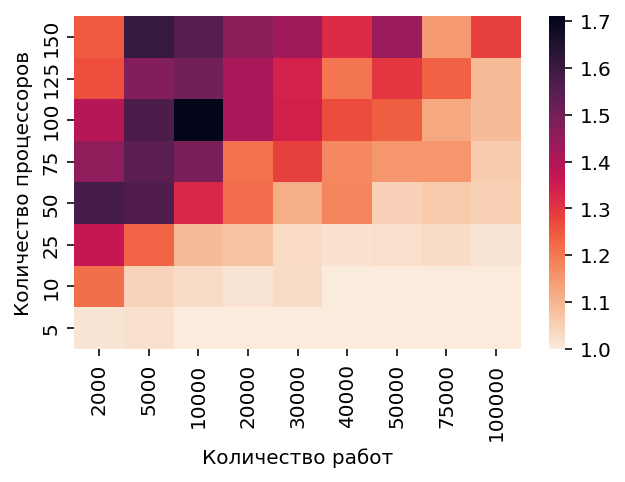
\includegraphics[width=\textwidth]{imgs/ideal_1/CR/th.png}
        \caption{Тепловая карта}
        \label{fig:CR-GC1-times-heatmap}
    \end{subfigure}
    \hfill
    \begin{subfigure}{0.49\textwidth}
        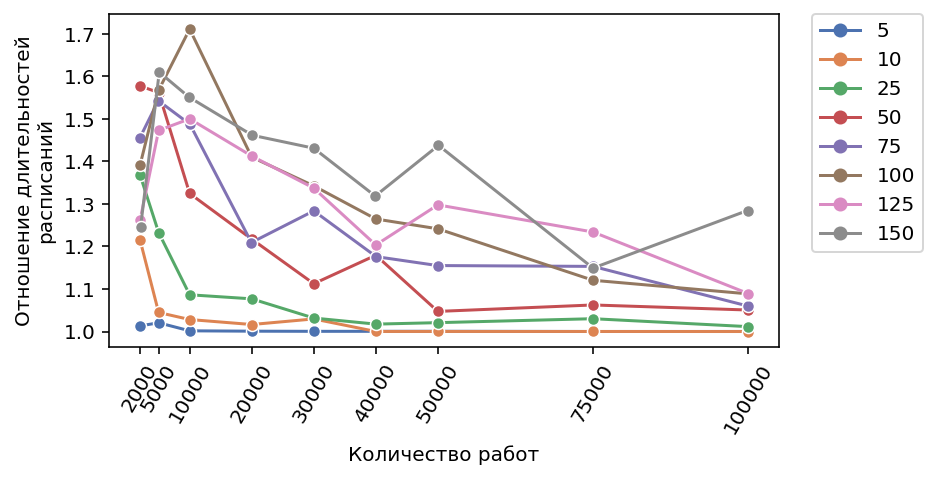
\includegraphics[width=\textwidth]{imgs/ideal_1/CR/gr_amalgamated.png}
        \caption{Сводный график}   
        \label{fig:CR-GC1-times-compiled} 
    \end{subfigure}
    \caption{Отношение времени выполнения расписания к оптимальному времени выполнения}
\end{figure}

На рисунках \ref{fig:CR-GC1-times-heatmap} и \ref{fig:CR-GC1-times-compiled} показано качество решений, генерируемых жадных алгоритмом с жадными критерием на данных с известным оптимумом. Цветом на рисунке \ref{fig:CR-GC1-times-heatmap} и значением на оси $Oy$ на рисунке \ref{fig:CR-GC1-times-compiled} показано отношение длительности расписания, построенного алгоритмом к длительности оптимального расписания. Значения всегда больше 1, чем меньше, тем лучше.

Точность алгоитма повышается с увеличением количества работ и уменьшается с повышением количества процессоров в системе. 

% \begin{figure}[!htbp]
%     \centering
%     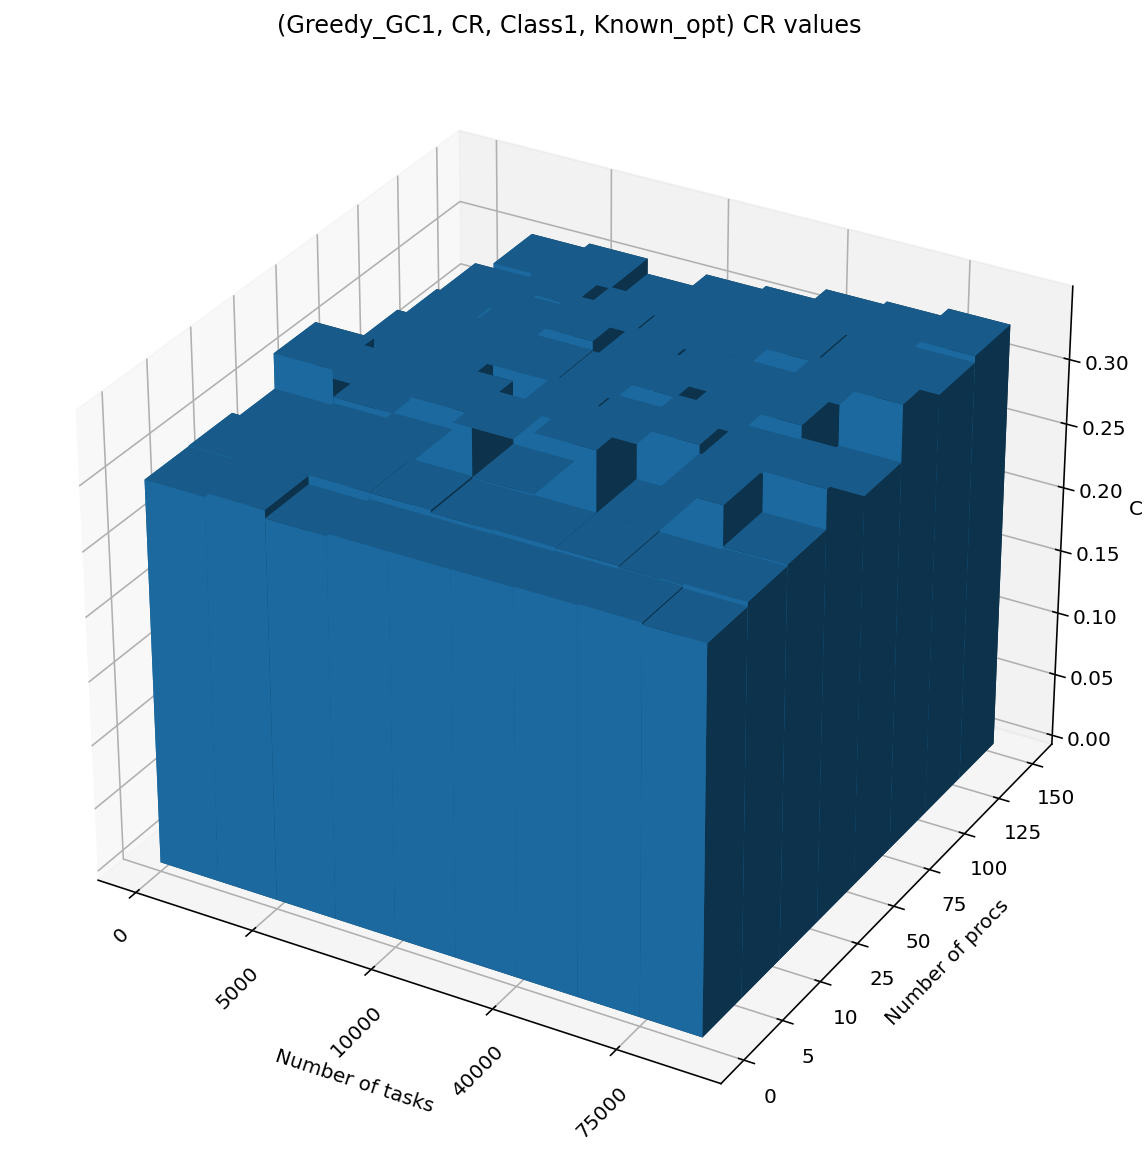
\includegraphics[width=\textwidth]{imgs/ideal_1/CR/cr_3d.png}
%     \caption{12345}
% \end{figure}

% \begin{figure}[!htbp]
%     \centering
%     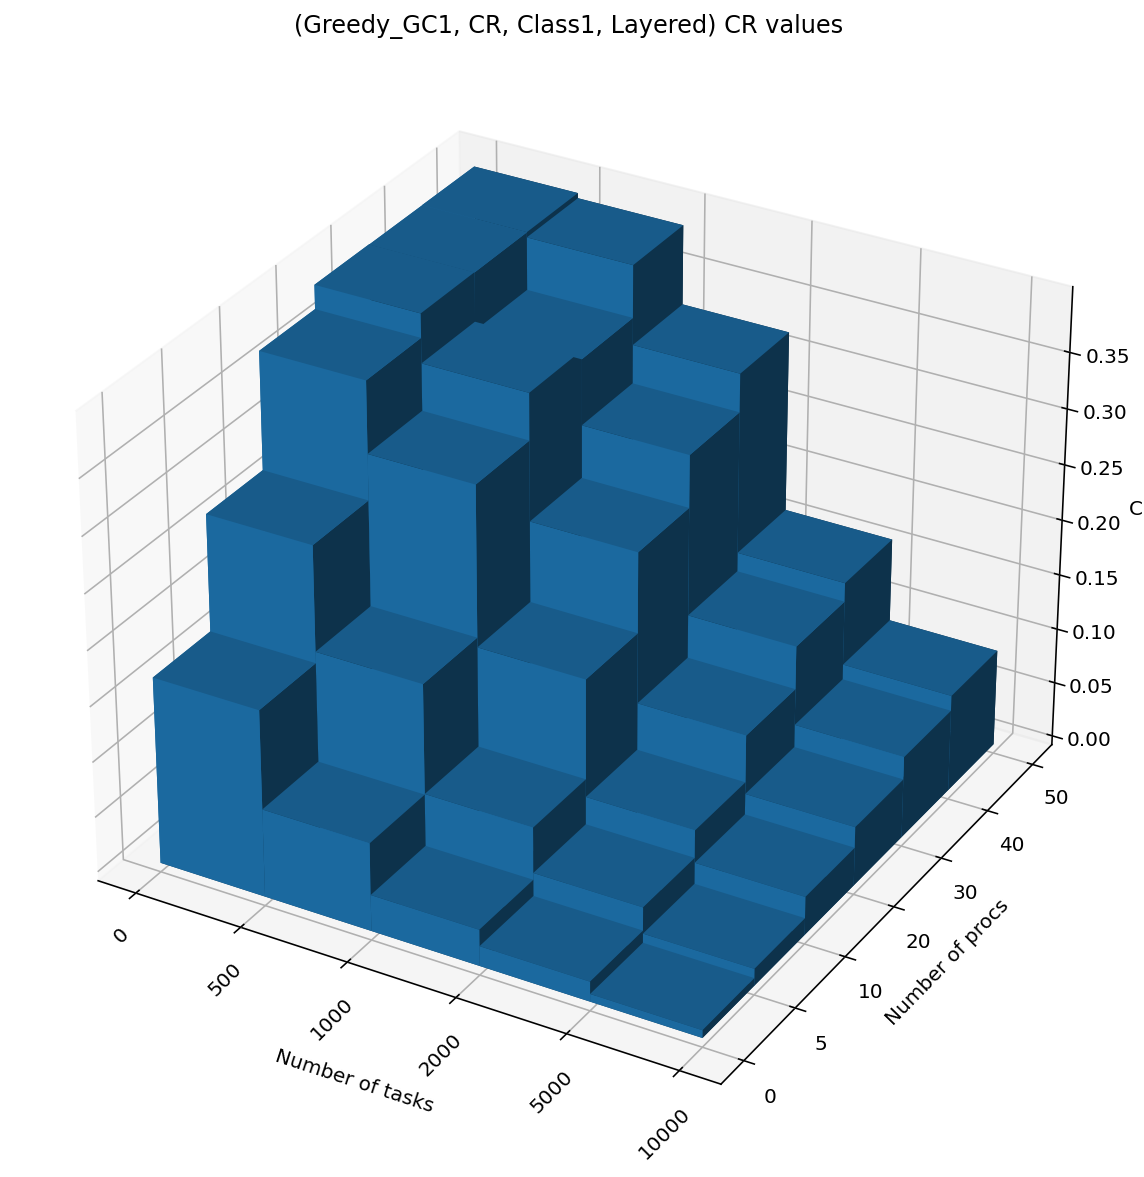
\includegraphics[width=\textwidth]{imgs/layered_class_1/CR/cr_3d.png}
%     \caption{12345}    
% \end{figure}

% \begin{figure}[!htbp]
%     \centering
%     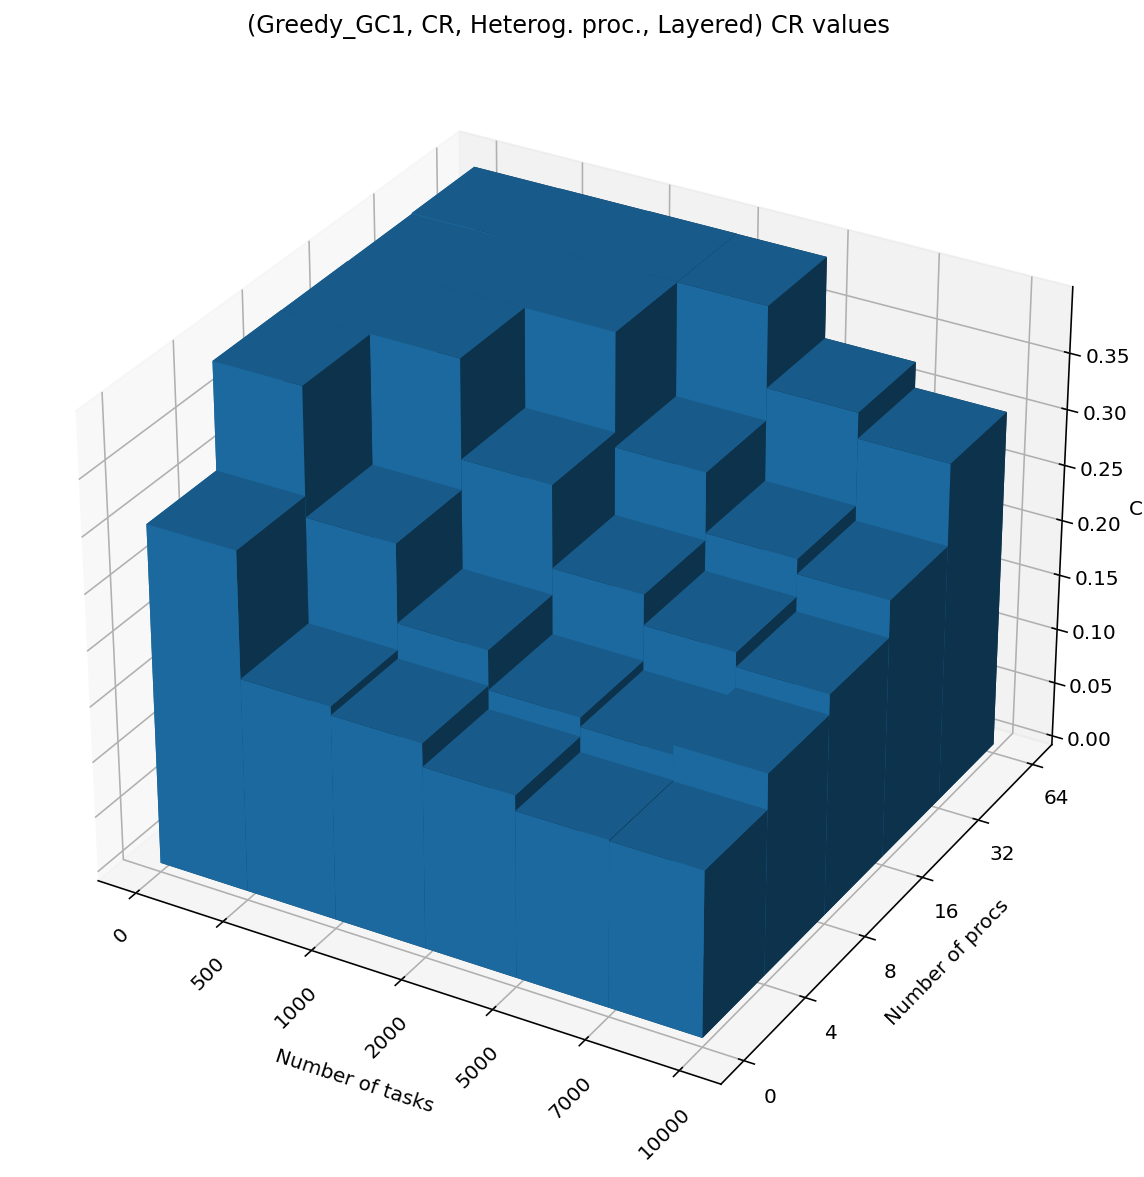
\includegraphics[width=\textwidth]{imgs/unbalanced/CR/cr_3d.png}
%     \caption{12345}
% \end{figure}

\paragraph{Постановка задачи без ограничений}

\begin{figure}[!htbp]
    \centering
    \begin{subfigure}{0.49\textwidth}
        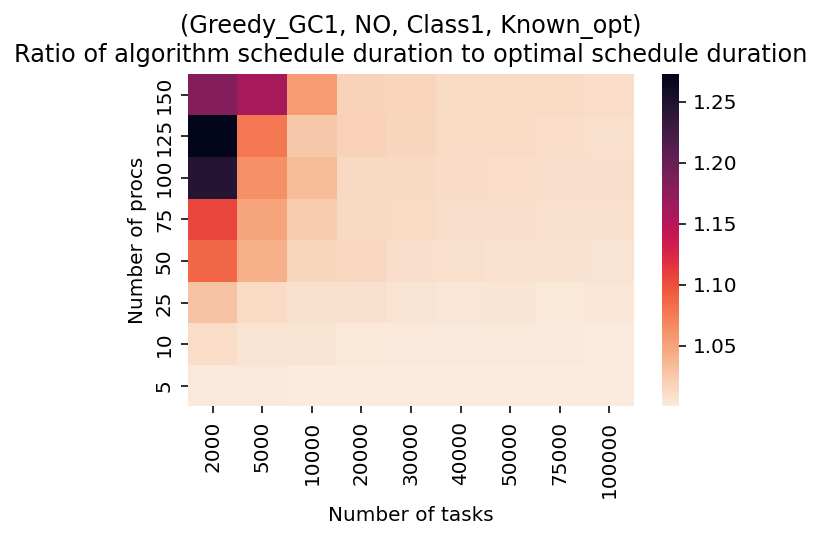
\includegraphics[width=\textwidth]{imgs/ideal_1/NO/th.png}
        \caption{Тепловая карта}   
        \label{fig:NO-GC1-times-heatmap}
    \end{subfigure}
    \hfill
    \begin{subfigure}{0.49\textwidth}
        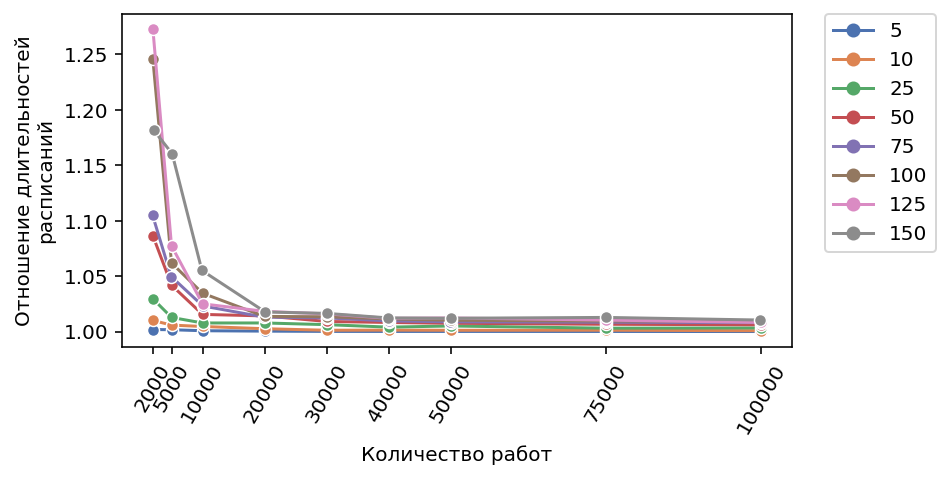
\includegraphics[width=\textwidth]{imgs/ideal_1/NO/gr_amalgamated.png}
        \caption{Сводный график}   
        \label{fig:NO-GC1-times-compiled} 
    \end{subfigure}
    \caption{Отношение времени выполнения расписания к оптимальному времени выполнения}
\end{figure}

На рисунках \ref{fig:NO-GC1-times-heatmap} и \ref{fig:NO-GC1-times-compiled} показано качество решенией, генерируемых жадных алгоритмом с жадными критерием на данных с известным оптимумом. Цветом на рисунке \ref{fig:NO-GC1-times-heatmap} и значением на оси $Oy$ на рисунке \ref{fig:NO-GC1-times-compiled} показано отношение длительности расписания, построенного алгоритмом к длительности оптимального расписания. Значения всегда больше 1, чем меньше, тем лучше.

Точность алгоритма возрастает с увеличением количества работ и понижается с увеличением количества процессоров.

\subsubsection{Жадный алгоритм с EDF эвристикой}

\paragraph{Постановка задачи с ограничением на количество передач}

\begin{figure}[!htbp]
    \centering
    \begin{subfigure}{0.49\textwidth}
        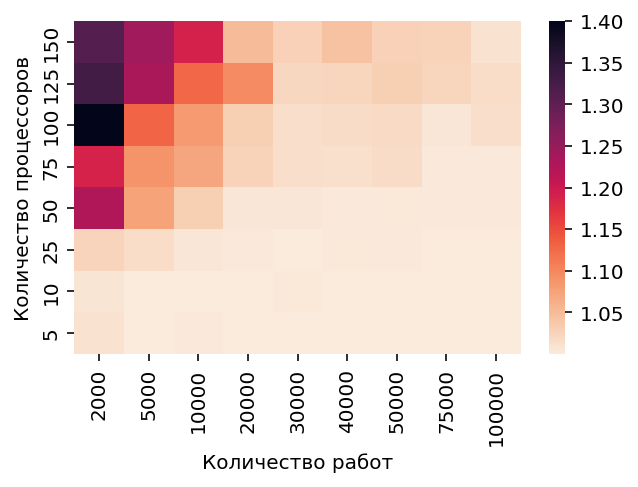
\includegraphics[width=\textwidth]{imgs/ideal_1/CR_EDF/th.png}
        \caption{Тепловая карта}
        \label{fig:CR-EDF-times-heatmap}
    \end{subfigure}
    \hfill
    \begin{subfigure}{0.49\textwidth}
        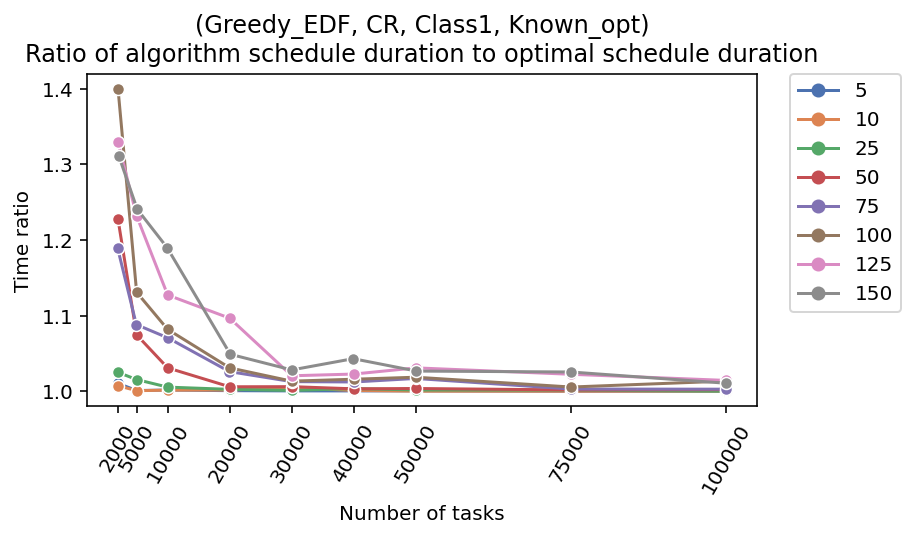
\includegraphics[width=\textwidth]{imgs/ideal_1/CR_EDF/gr_amalgamated.png}
        \caption{Сводный график} 
        \label{fig:CR-EDF-times-compiled} 
    \end{subfigure}
    \caption{Отношение времени выполнения расписания к оптимальному времени выполнения}
\end{figure}

На рисунках \ref{fig:CR-EDF-times-heatmap} и \ref{fig:CR-EDF-times-compiled} показано качество решенией, генерируемых жадным алгоритмом с жадными критерием на данных с известным оптимумом. Цветом на рисунке \ref{fig:CR-EDF-times-heatmap} и значением на оси $Oy$ на рисунке \ref{fig:CR-EDF-times-compiled} показано отношение длительности расписания, построенного алгоритмом к длительности оптимального расписания. Значения всегда больше 1, чем меньше, тем лучше.

Точность алгоритма повышается с увеличением количества работ, однако ухудшение решения с увеличением количества процессоров в системе менее значительно, чем в жадном алгоритме. 

% \begin{figure}[!htbp]
%     \centering
%     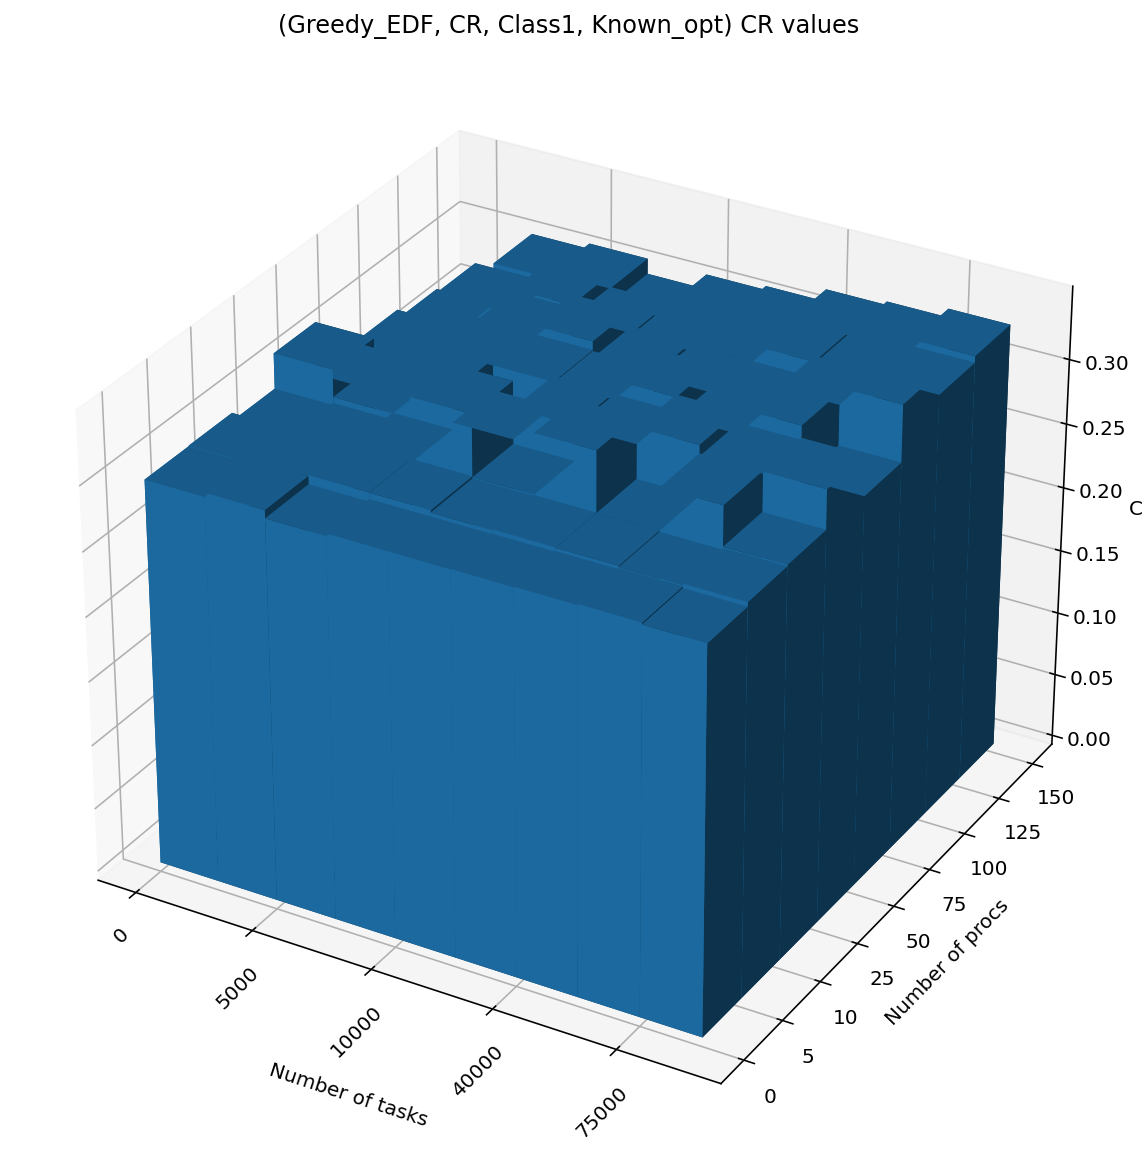
\includegraphics[width=\textwidth]{imgs/ideal_1/CR_EDF/cr_3d.png}
%     \caption{12345}
% \end{figure}

\begin{figure}[!htbp]
    \centering
    \begin{subfigure}{0.49\textwidth}
        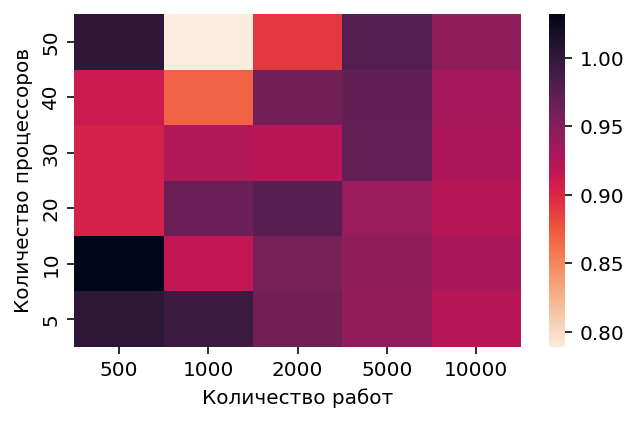
\includegraphics[width=\textwidth]{imgs/layered_class_1/CR_EDF/times.png}
        \caption{Тепловая карта}
        \label{fig:CR-layered-EDF-times-heatmap}
    \end{subfigure}
    \hfill
    \begin{subfigure}{0.49\textwidth}
        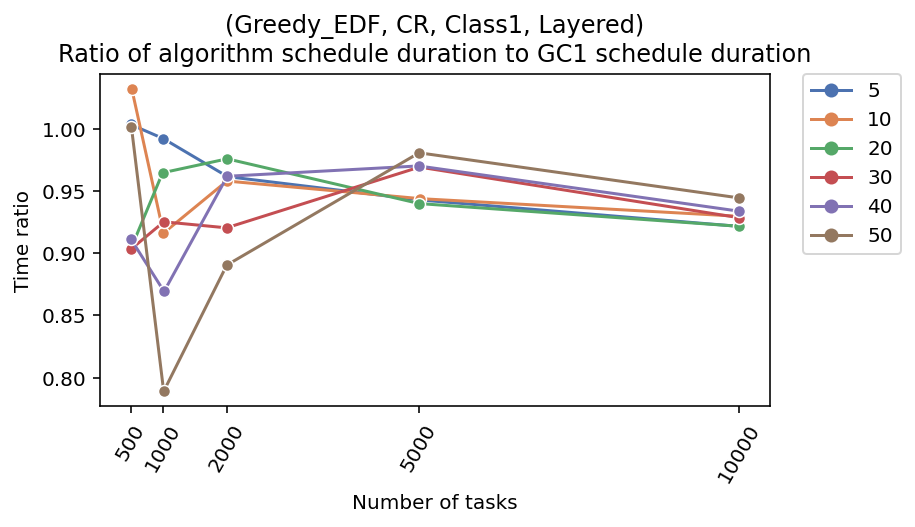
\includegraphics[width=\textwidth]{imgs/layered_class_1/CR_EDF/gr_amalgamated.png}
        \caption{Сводный график}
        \label{fig:CR-layered-EDF-times-compiled} 
    \end{subfigure}
    \caption{Отношение времени выполнения расписания к времени выполнения расписания, построенного при помощи жадного алгоритма}
\end{figure}

На рисунках \ref{fig:CR-layered-EDF-times-heatmap} и \ref{fig:CR-layered-EDF-times-compiled} показано качество решений, генерируемых жадным алгоритмом с EDF эвристикой на данных, построенных на слоистых графах. Цветом на рисунке \ref{fig:CR-layered-EDF-times-heatmap} и значением на оси $Oy$ на рисунке \ref{fig:CR-layered-EDF-times-compiled} показано отношение длительности расписании расписании, построенного жадным алгоритмом с жадным кртерием.

В большинстве случаев, качество решений жадного алгоритма с EDF эвристикой лучше качества решений жадного лагоритма, однако преимущество остается в пределах 10\%, кроме двух выбросов в районе 1000 работ. 

% \begin{figure}[!htbp]
%     \centering
%     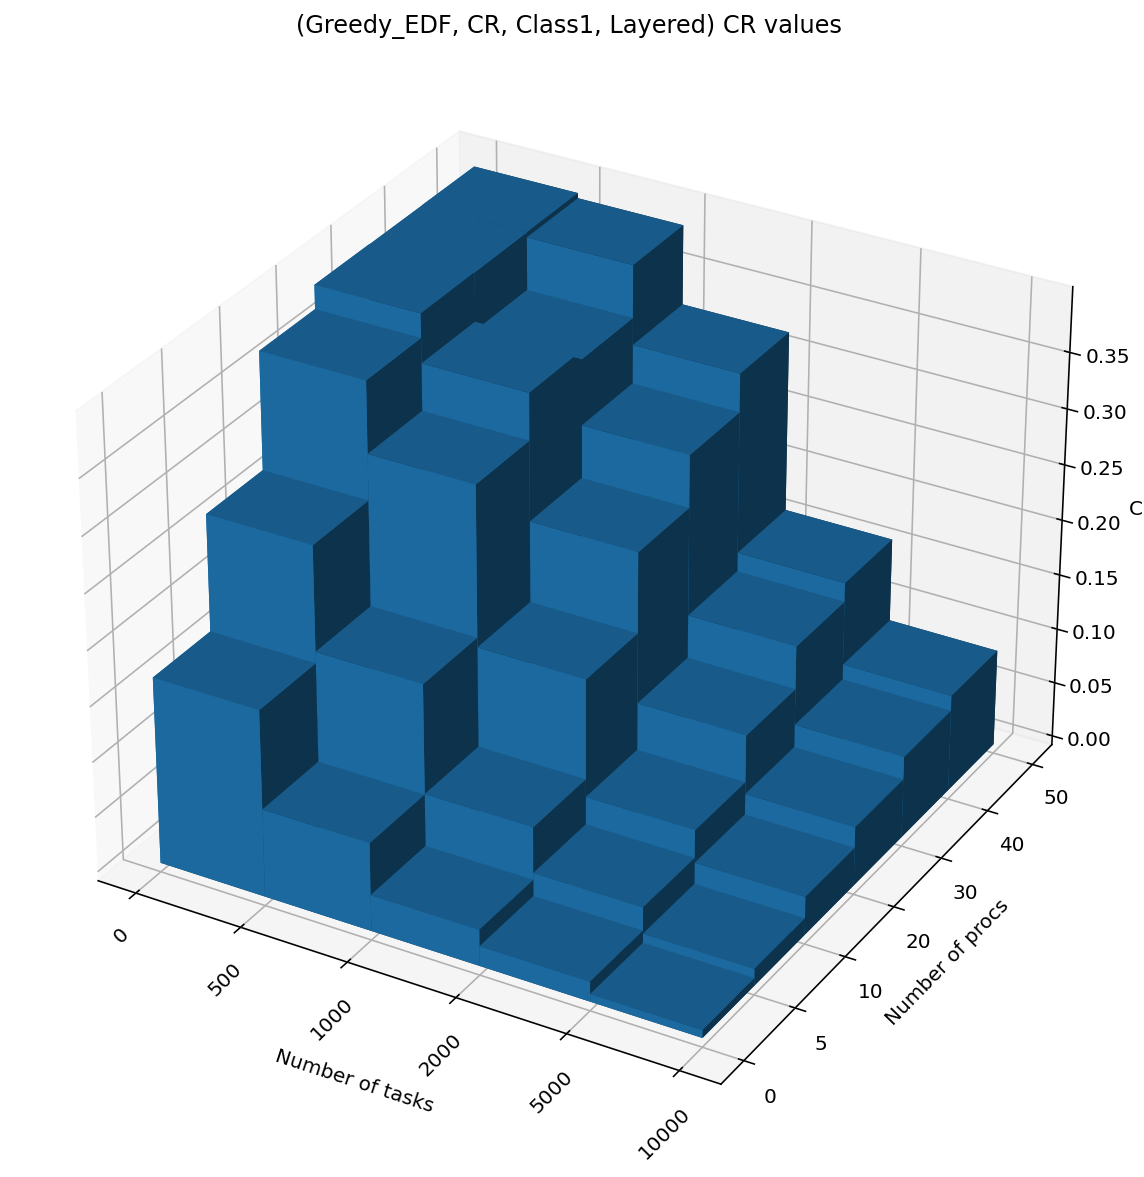
\includegraphics[width=\textwidth]{imgs/layered_class_1/CR_EDF/cr_3d.png}
%     \caption{12345}
% \end{figure}

\begin{figure}[!htbp]
    \centering
    \begin{subfigure}{0.49\textwidth}
        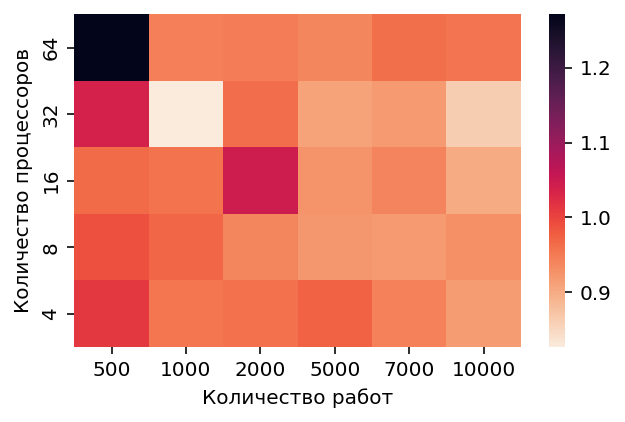
\includegraphics[width=\textwidth]{imgs/unbalanced/CR_EDF/times.png}
        \caption{Тепловая карта}
        \label{fig:CR-disbalanced-EDF-times-heatmap}
    \end{subfigure}
    \hfill
    \begin{subfigure}{0.49\textwidth}
        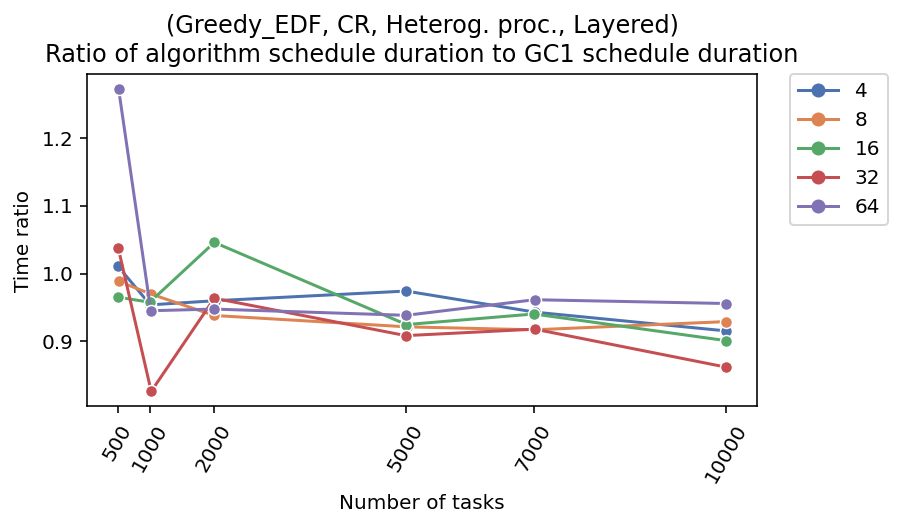
\includegraphics[width=\textwidth]{imgs/unbalanced/CR_EDF/gr_amalgamated.png}
        \caption{Сводный график}
        \label{fig:CR-disbalanced-EDF-times-compiled} 
    \end{subfigure}
    \caption{Отношение времени выполнения расписания к времени выполнения расписания, построенного при помощи жадного алгоритма}
\end{figure}

На рисунках \ref{fig:CR-disbalanced-EDF-times-heatmap} и \ref{fig:CR-disbalanced-EDF-times-compiled} показано качество решений, генерируемых жадным алгоритмом с EDF эвристикой на данных, построенных на слоистых графах. Цветом на рисунке \ref{fig:CR-disbalanced-EDF-times-heatmap} и значением на оси $Oy$ на рисунке \ref{fig:CR-disbalanced-EDF-times-compiled} показано отношение длительности расписании расписании, построенного жадным алгоритмом с жадным кртерием.

Алгоритм не дает значимых улучшений решения по сравнению с жадным алгоритмом, кроме случая с 500 работами на 64 процессорах, в котром решение, строимое жадным алгоритмом с EDF эвристикой значительно хуже решения, построенного жадным алгоритмом.

% \begin{figure}[!htbp]
%     \centering
%     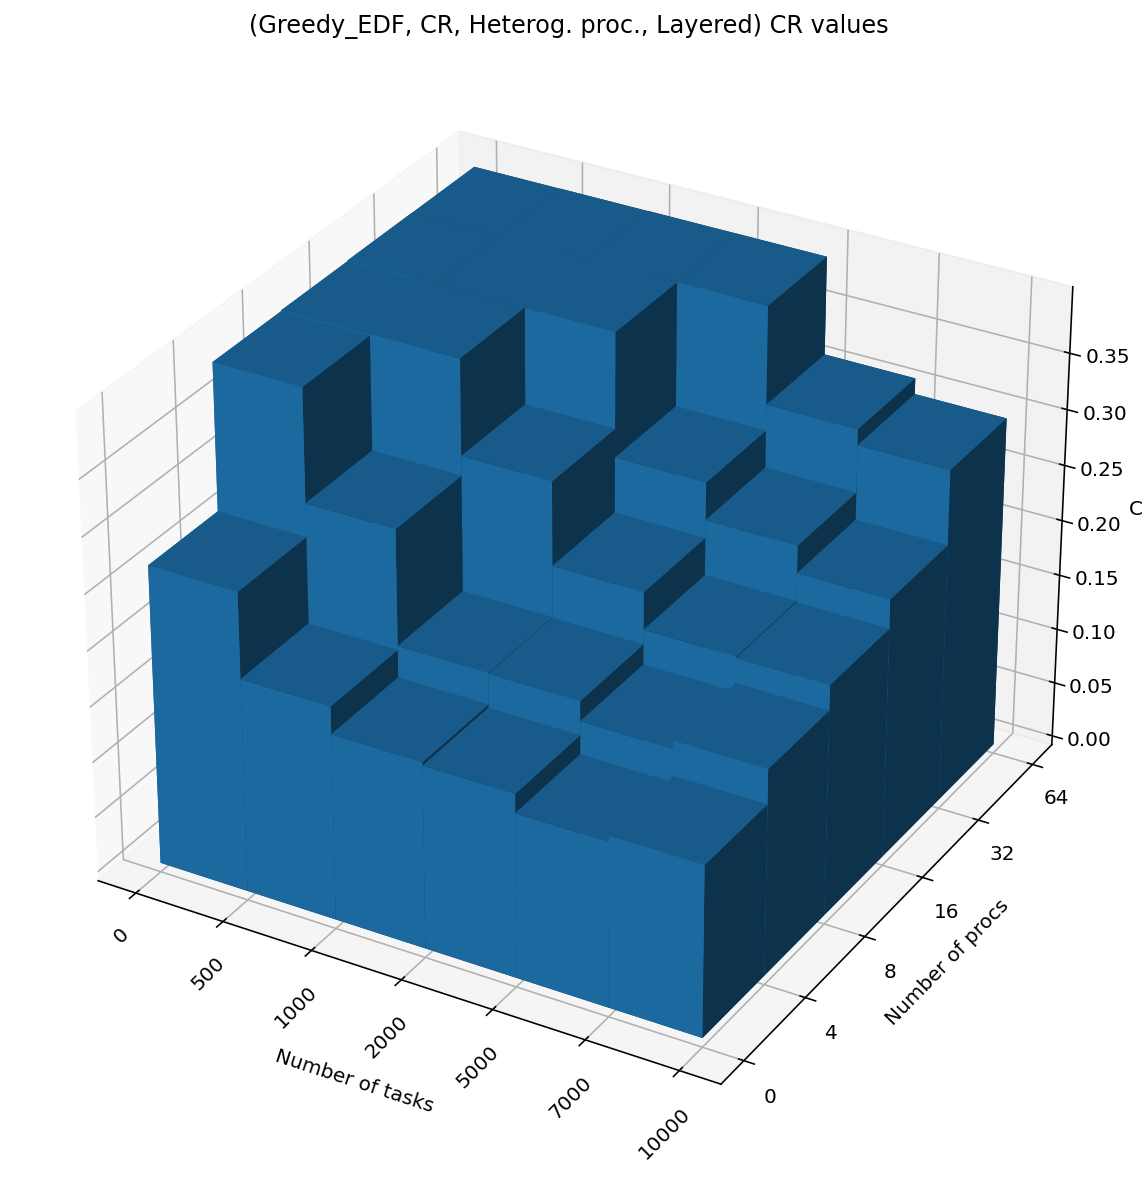
\includegraphics[width=\textwidth]{imgs/unbalanced/CR_EDF/cr_3d.png}
%     \caption{12345}
% \end{figure}

\paragraph{Постановка задачи без ограничений}

\begin{figure}[!htbp]
    \centering
    \begin{subfigure}{0.49\textwidth}
        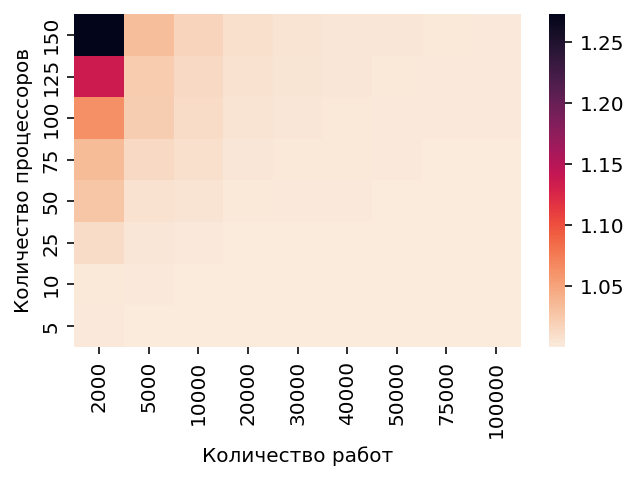
\includegraphics[width=\textwidth]{imgs/ideal_1/NO_EDF/th.png}
        \caption{Тепловая карта}
        \label{fig:NO-EDF-times-heatmap}
    \end{subfigure}
    \hfill
    \begin{subfigure}{0.49\textwidth}
        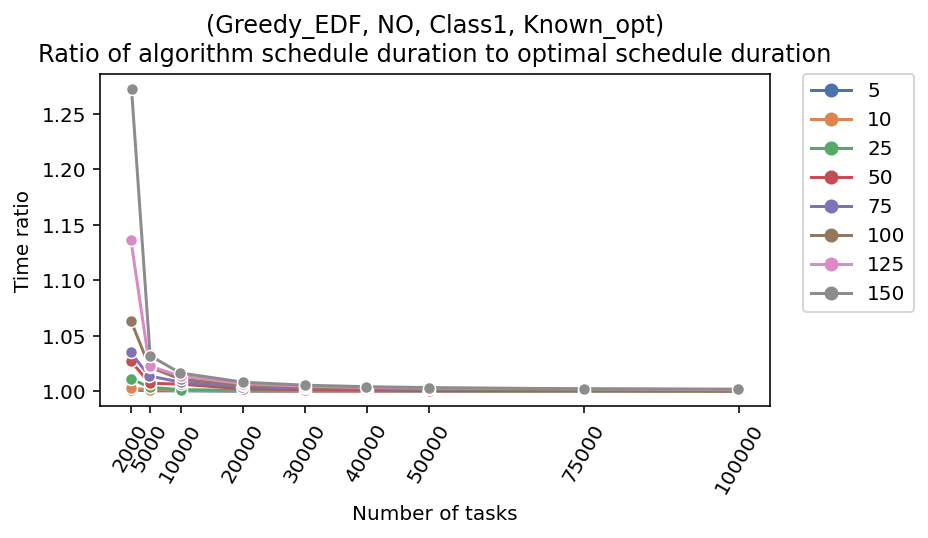
\includegraphics[width=\textwidth]{imgs/ideal_1/NO_EDF/gr_amalgamated.png}
        \caption{Сводный график} 
        \label{fig:NO-EDF-times-compiled}
    \end{subfigure}
    \caption{Отношение времени выполнения расписания к оптимальному времени выполнения}
\end{figure}

На рисунках \ref{fig:NO-EDF-times-heatmap} и \ref{fig:NO-EDF-times-compiled} показано качество решений, генерируемых жадным алгоритмом с EDF эвристикой на данных с известным оптимумом. Цветом на рисунке \ref{fig:NO-EDF-times-heatmap} и значением на оси $Oy$ на рисунке \ref{fig:NO-EDF-times-compiled} показано отношение длительности расписания, построенного жадным алгоритмом с жадным кртерием. Значения всегда больше 1, чем меньше, тем лучше.

Алгоритм хорошо справляется с задачей, в большинстве случаев отклонение от оптимума не превышает 5\%. Для 2000 и 5000 работ точность алгоритма значительно выше таковой для жадного алгоритма.

\begin{figure}[!htbp]
    \centering
    \begin{subfigure}{0.49\textwidth}
        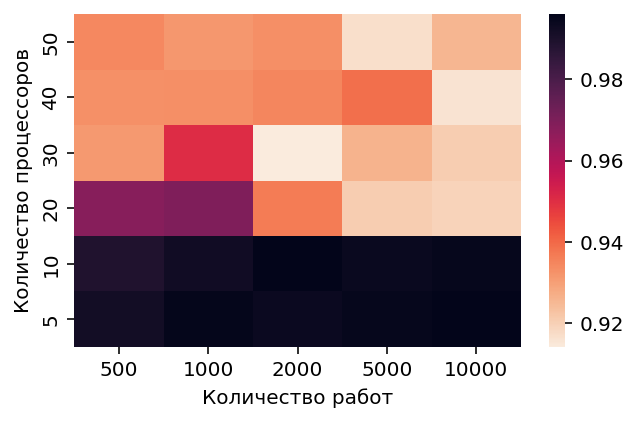
\includegraphics[width=\textwidth]{imgs/layered_class_1/NO_EDF/times.png}
        \caption{Тепловая карта}
        \label{fig:NO-layered-EDF-times-heatmap}
    \end{subfigure}
    \hfill
    \begin{subfigure}{0.49\textwidth}
        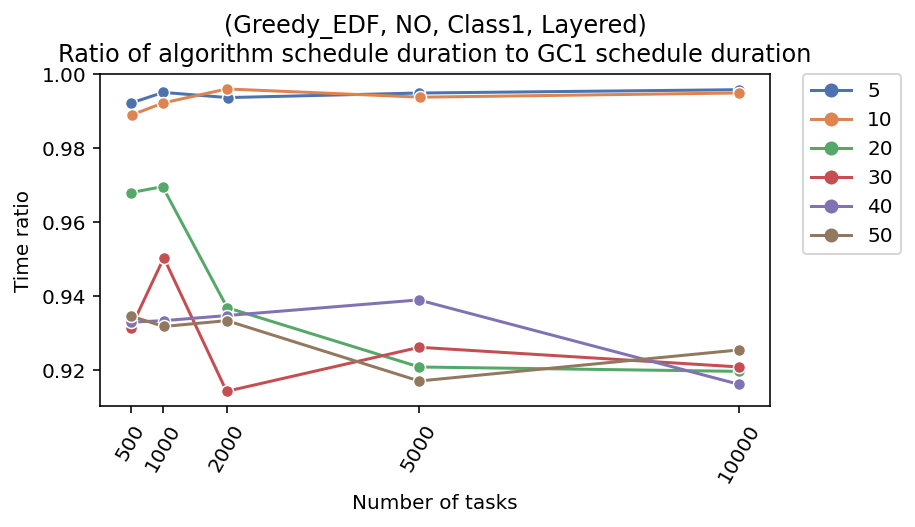
\includegraphics[width=\textwidth]{imgs/layered_class_1/NO_EDF/gr_amalgamated.png}
        \caption{Сводный график} 
        \label{fig:NO-layered-EDF-times-compiled}
    \end{subfigure}
    \caption{Отношение времени выполнения расписания к оптимальному времени выполнения}
\end{figure}

На рисунках \ref{fig:NO-layered-EDF-times-heatmap} и \ref{fig:NO-layered-EDF-times-compiled} показано качество решений, генерируемых жадным алгоритмом с EDF эвристикой на данных, построенных на слоистых графах. Цветом на рисунке \ref{fig:NO-layered-EDF-times-heatmap} и значением на оси $Oy$ на рисунке \ref{fig:NO-layered-EDF-times-compiled} показано отношение длительности расписания, построенного жадным алгоритмом с жадным кртерием.

Во всех случаях, качество решений выше качетва решений жадного алгоритма, но это улучшение не превышает 10\%.

\begin{figure}[!htbp]
    \centering
    \begin{subfigure}{0.49\textwidth}
        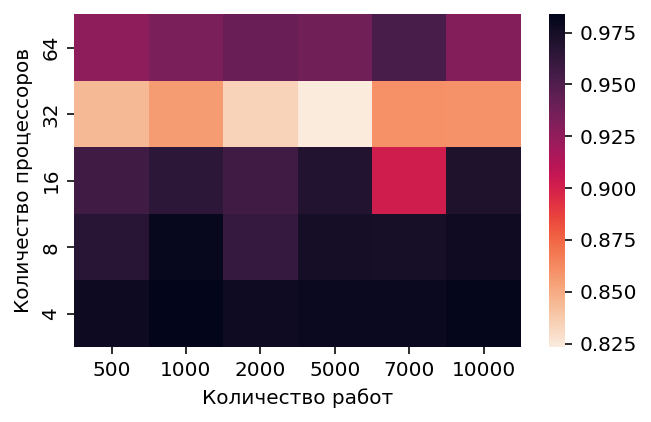
\includegraphics[width=\textwidth]{imgs/unbalanced/NO_EDF/times.png}
        \caption{Тепловая карта}
        \label{fig:NO-disbalanced-EDF-times-heatmap}
    \end{subfigure}
    \hfill
    \begin{subfigure}{0.49\textwidth}
        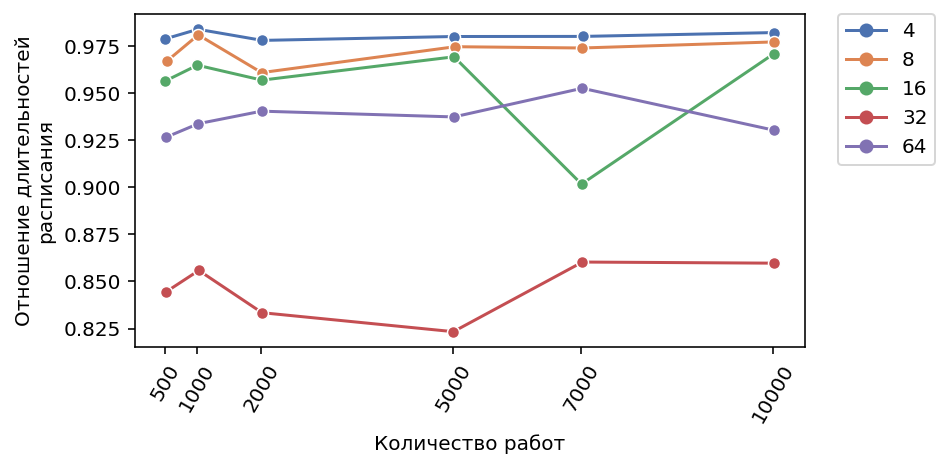
\includegraphics[width=\textwidth]{imgs/unbalanced/NO_EDF/gr_amalgamated.png}
        \caption{Сводный график}
        \label{fig:NO-disbalanced-EDF-times-compiled}
    \end{subfigure}
    \caption{Отношение времени выполнения расписания к времени выполнения расписания, построенного при помощи жадного алгоритма}
\end{figure}

На рисунках \ref{fig:NO-disbalanced-EDF-times-heatmap} и \ref{fig:NO-disbalanced-EDF-times-compiled} показано качество решений, генерируемых жадным алгоритмом с EDF эвристикой на данных, построенных на слоистых графах. Цветом на рисунке \ref{fig:NO-disbalanced-EDF-times-heatmap} и значением на оси $Oy$ на рисунке \ref{fig:NO-disbalanced-EDF-times-compiled} показано отношение длительности расписании расписании, построенного жадным алгоритмом с жадным кртерием. Значения всегда больше 1, чем меньше, тем лучше.

Во всех случаях, качество решений выше качетва решений жадного алгоритма, но это улучшение не превышает 10\%, за исключением случая с 32 процессорами.

\subsection{Исследование временной сложности алгоритма}

\subsubsection{Жадный алгоритм}

\paragraph{Постановка задачи с ограничением на количество передач}

\begin{figure}[!htbp]
    \centering
    \begin{subfigure}{0.49\textwidth}
        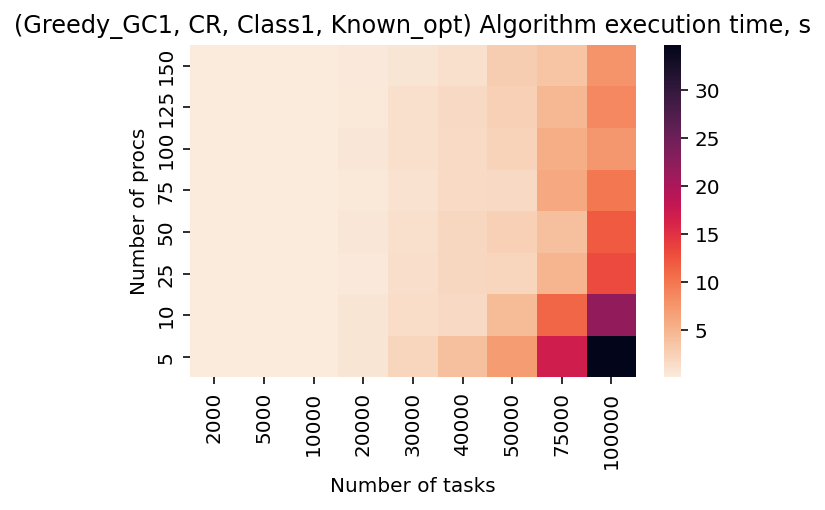
\includegraphics[width=\textwidth]{imgs/ideal_1/CR/et_heatmap.png}
        \caption{Тепловая карта}
        \label{fig:CR-exec-time-heatmap}
    \end{subfigure}
    \hfill
    \begin{subfigure}{0.49\textwidth}
        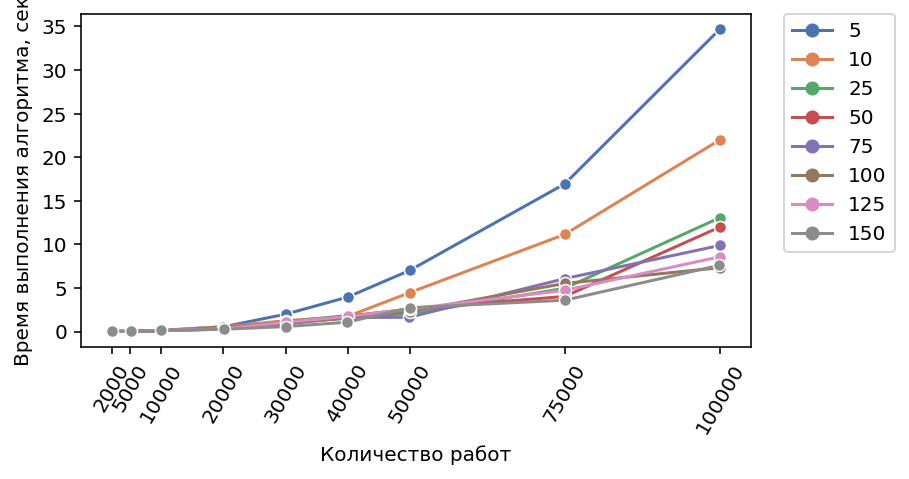
\includegraphics[width=\textwidth]{imgs/ideal_1/CR/tr_graph.png}
        \caption{Сводный график}
        \label{fig:CR-exec-time-compiled}
    \end{subfigure}
    \caption{Время выполнения алгоритма, в секундах}
\end{figure}

На рисунках \ref{fig:CR-exec-time-heatmap} и \ref{fig:CR-exec-time-compiled} показано время выполнения жадного алгоритма, включая прогоны METIS. Время выполнения растет с увеличением количества вершин. При равном количестве работ, выше время выполнения при меньшем количестве процессоров. Причина в том, что при равном количестве работ и понижении количества процессоров повышается количество работ, распределенных на процессор, что приводит к большему количеству пропусков в расписании, что значит, что алгоритм постановки работы в расписании отработает быстрее, т.к. он работает до первого найденного доступного простоя на процессоре. 

\begin{figure}[!htbp]
    \centering
    \begin{subfigure}{0.49\textwidth}
        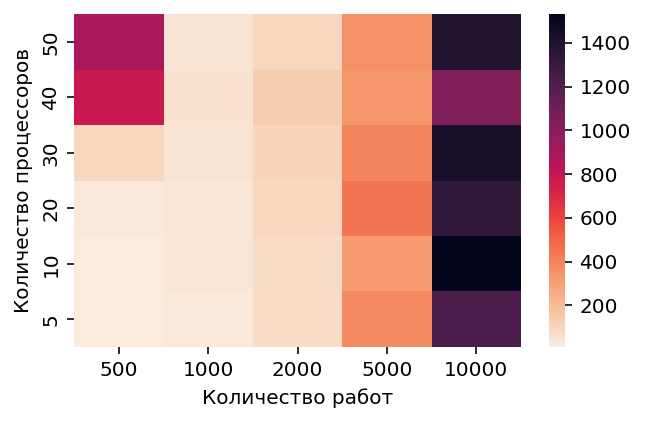
\includegraphics[width=\textwidth]{imgs/layered_class_1/CR/et_heatmap.png}
        \caption{Тепловая карта}
        \label{fig:CR-layered-exec-time-heatmap}
    \end{subfigure}
    \hfill
    \begin{subfigure}{0.49\textwidth}
        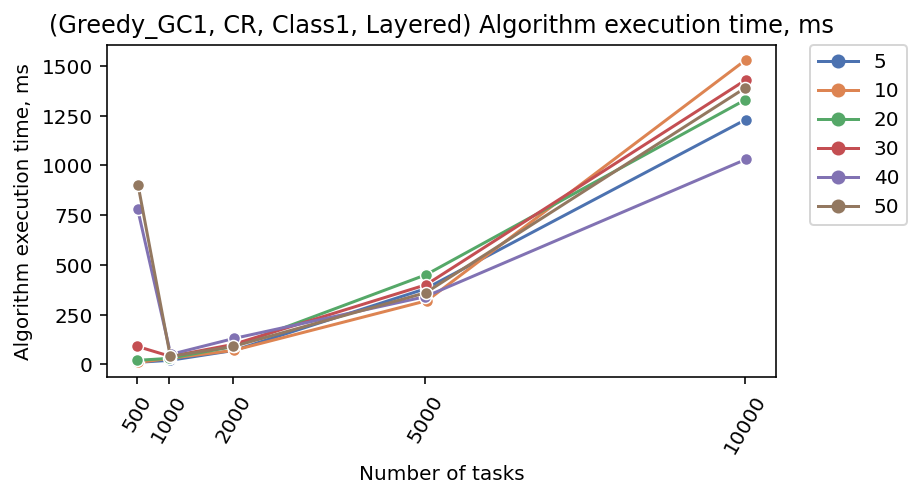
\includegraphics[width=\textwidth]{imgs/layered_class_1/CR/tr_graph.png}
        \caption{Сводный график}
        \label{fig:CR-layered-exec-time-compiled}
    \end{subfigure}
    \caption{Время выполнения алгоритма, в миллисекундах}
\end{figure}

На рисунках \ref{fig:CR-layered-exec-time-heatmap} и \ref{fig:CR-layered-exec-time-compiled} показано время выполнения алгоритма на наборе данных, основанных на слоистых графах. 

Кроме двух выбросов, соотносящихся с самым малым количеством работ и самым большим количеством процессоров в системе, нет существенной зависимости времени выполнения от количества процессоров в системе.

\begin{figure}[!htbp]
    \centering
    \begin{subfigure}{0.49\textwidth}
        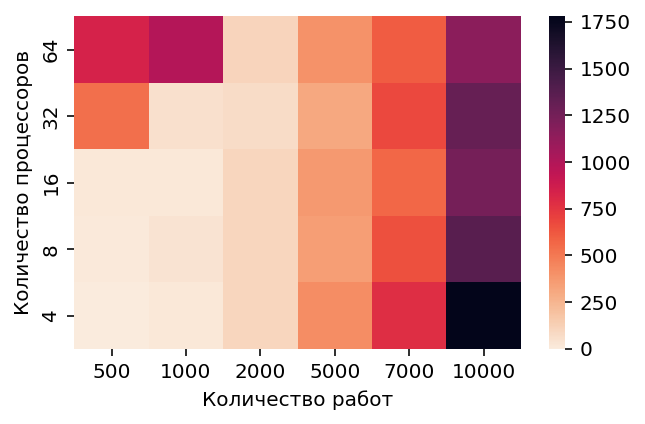
\includegraphics[width=\textwidth]{imgs/unbalanced/CR/et_heatmap.png}
        \caption{Тепловая карта}
        \label{fig:CR-disbalanced-exec-time-heatmap}
    \end{subfigure}
    \hfill
    \begin{subfigure}{0.49\textwidth}
        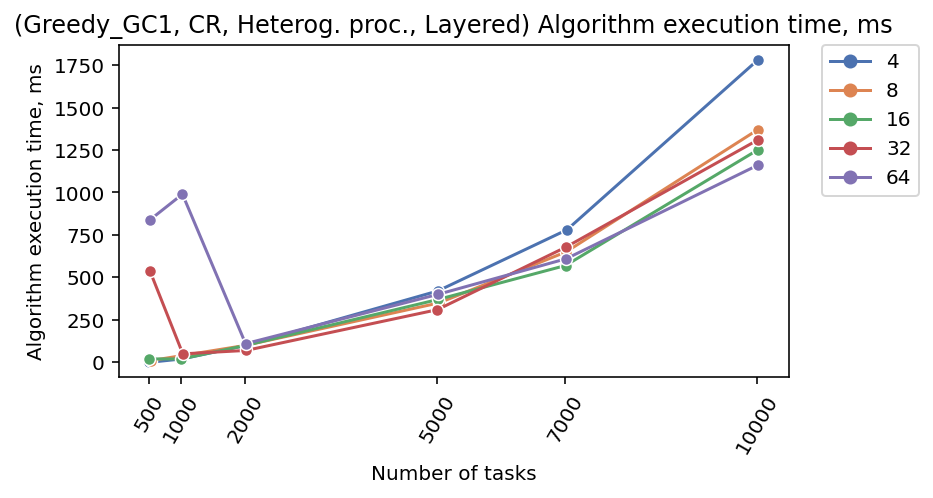
\includegraphics[width=\textwidth]{imgs/unbalanced/CR/tr_graph.png}
        \caption{Сводный график}
        \label{fig:CR-disbalanced-exec-time-compiled}
    \end{subfigure}
    \caption{Время выполнения алгоритма, в миллисекундах}
\end{figure}

На рисунках \ref{fig:CR-disbalanced-exec-time-heatmap} и \ref{fig:CR-disbalanced-exec-time-compiled} показано время выполнения алгоритма на наборе данных, основанных на слоистых графах с неоднородными процессорами.

Время выполнения алгоритма растет с увеличением количества работ, кроме трех выбросов. Эти выбросы соответствуют самому малому количеству работ и самому высокому количеству процессоров.

\paragraph{Постановка задачи без ограничений}

\begin{figure}[!htbp]
    \centering
    \begin{subfigure}{0.49\textwidth}
        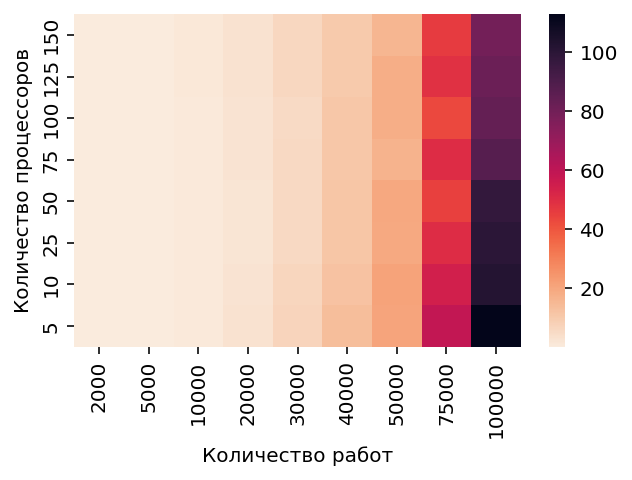
\includegraphics[width=\textwidth]{imgs/ideal_1/NO/et_heatmap.png}
        \caption{Тепловая карта}
        \label{fig:NO-exec-time-heatmap}
    \end{subfigure}
    \hfill
    \begin{subfigure}{0.49\textwidth}
        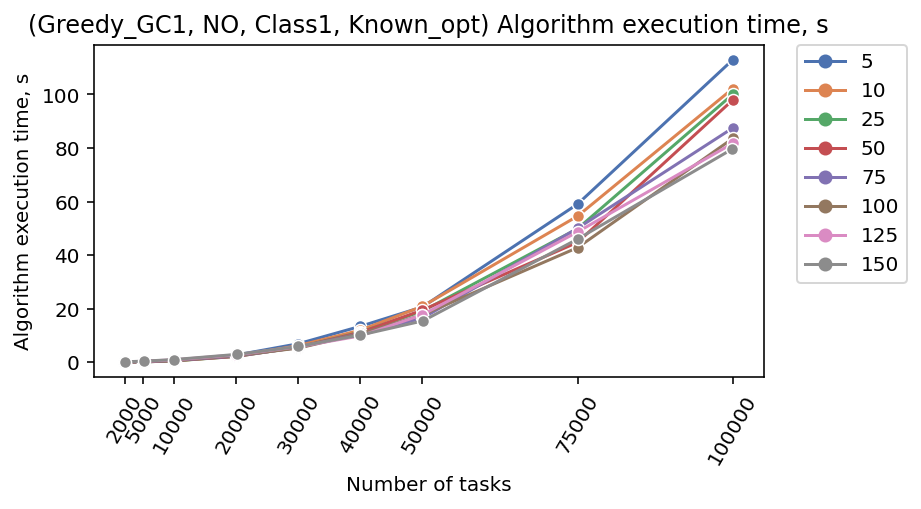
\includegraphics[width=\textwidth]{imgs/ideal_1/NO/tr_graph.png}
        \caption{Сводный график}
        \label{fig:NO-exec-time-compiled}
    \end{subfigure}
    \caption{Время выполнения алгоритма, в секундах}
\end{figure}

На рисунках \ref{fig:NO-exec-time-heatmap} и \ref{fig:NO-exec-time-compiled} показано время выполнения алгоритма на наборе данных c известным оптимумом. Время выполнения растет с увеличением количества задач. 

При одинаковом количестве работ, быстрее выполняется алгоритм с большим количеством процессоров, по тем же причинами, что и в постановке с дополнительным ограничением $CR$. 

\begin{figure}[!htbp]
    \centering
    \begin{subfigure}{0.49\textwidth}
        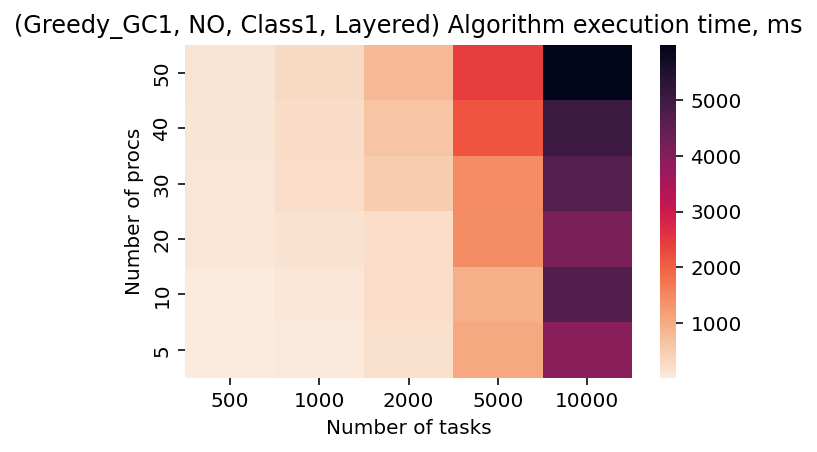
\includegraphics[width=\textwidth]{imgs/layered_class_1/NO/et_heatmap.png}
        \caption{Тепловая карта}
        \label{fig:NO-layered-exec-time-heatmap}
    \end{subfigure}
    \hfill
    \begin{subfigure}{0.49\textwidth}
        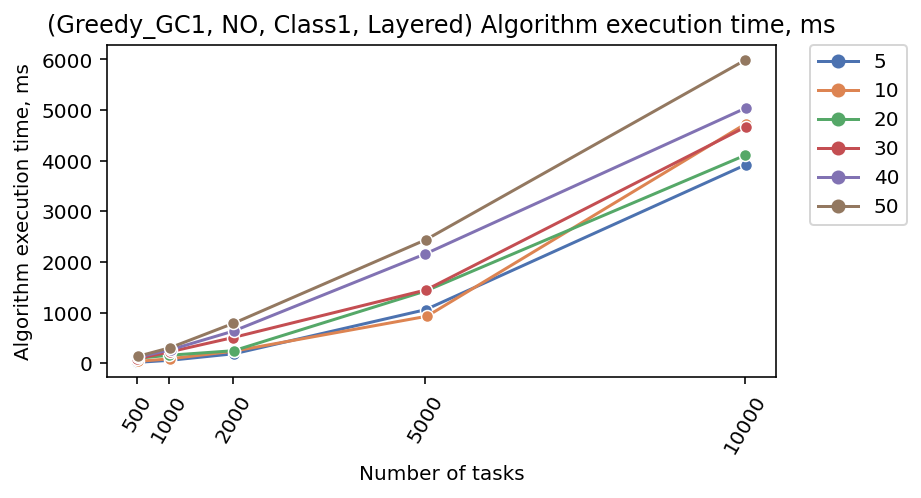
\includegraphics[width=\textwidth]{imgs/layered_class_1/NO/tr_graph.png}
        \caption{Сводный график}
        \label{fig:NO-layered-exec-time-compiled}
    \end{subfigure}
    \caption{Время выполнения алгоритма, в миллисекундах}
\end{figure}

На рисунках \ref{fig:NO-exec-time-heatmap} и \ref{fig:NO-exec-time-compiled} показано время выполнения алгоритма на наборе данных, основанных на слоистых графах. Время выполнения растет с увеличением количества работ и количества процессоров.

\begin{figure}[!htbp]
    \centering
    \begin{subfigure}{0.49\textwidth}
        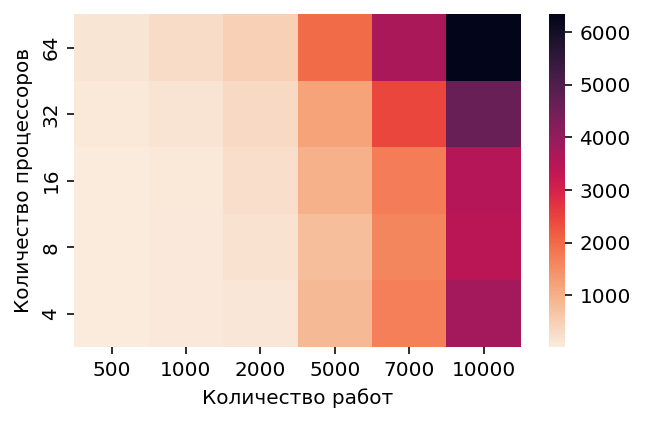
\includegraphics[width=\textwidth]{imgs/unbalanced/NO/et_heatmap.png}
        \caption{Тепловая карта}
        \label{fig:NO-unbalanced-exec-time-heatmap}
    \end{subfigure}
    \hfill
    \begin{subfigure}{0.49\textwidth}
        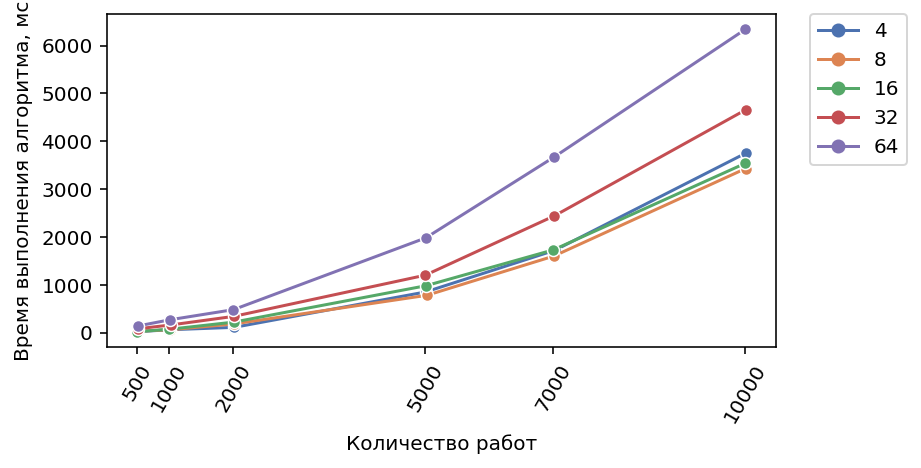
\includegraphics[width=\textwidth]{imgs/unbalanced/NO/tr_graph.png}
        \caption{Сводный график}
        \label{fig:NO-unbalanced-exec-time-compiled}
    \end{subfigure}
    \caption{Время выполнения алгоритма, в миллисекундах}
\end{figure}

На рисунках \ref{fig:NO-unbalanced-exec-time-heatmap} и \ref{fig:NO-unbalanced-exec-time-compiled} показано время выполнения алгоритма на наборе данных c неоднородными процессорами. Время выполнения растет с увеличением количества работ и количества процессоров.

\subsubsection{Жадный алгоритм с EDF эвристикой}

\paragraph{Постановка задачи с ограничением на количество передач}

\begin{figure}[!htbp]
    \centering
    \begin{subfigure}{0.49\textwidth}
        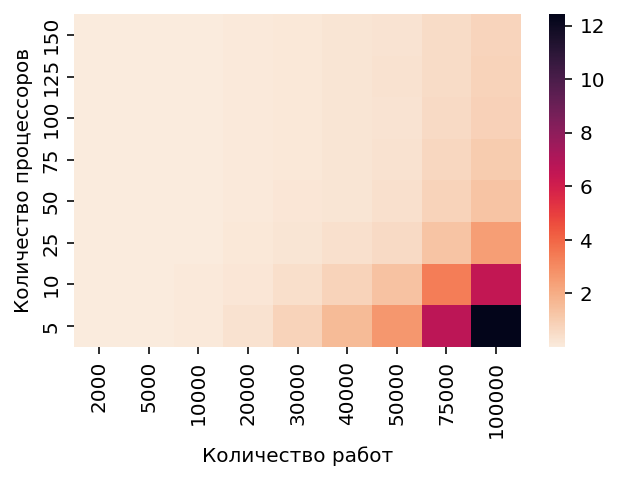
\includegraphics[width=\textwidth]{imgs/ideal_1/CR_EDF/et_heatmap.png}
        \caption{Тепловая карта}
        \label{fig:CR-EDF-exec-time-heatmap}
    \end{subfigure}
    \hfill
    \begin{subfigure}{0.49\textwidth}
        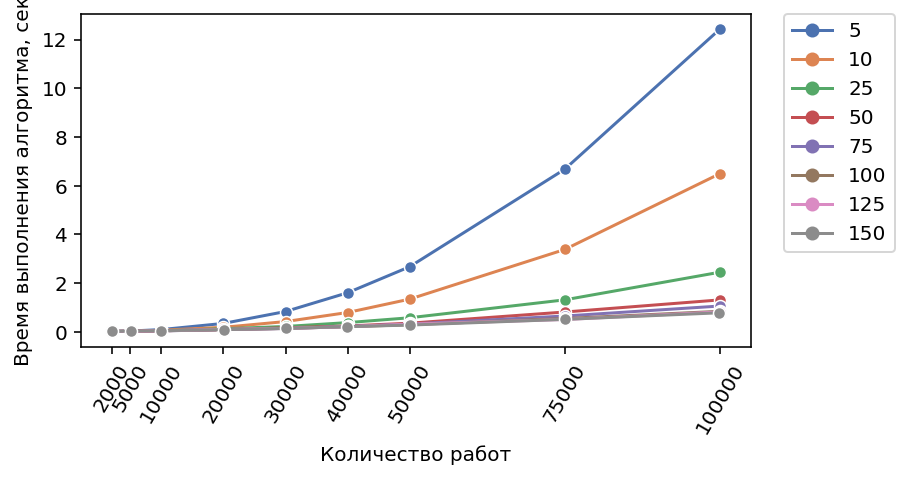
\includegraphics[width=\textwidth]{imgs/ideal_1/CR_EDF/tr_graph.png}
        \caption{Сводный график}
        \label{fig:CR-EDF-exec-time-compiled}
    \end{subfigure}
    \caption{Время выполнения алгоритма, в секундах}
\end{figure}

На рисунках \ref{fig:CR-EDF-exec-time-heatmap} и \ref{fig:CR-EDF-exec-time-compiled} показано время выполнения жадного алгоритма с EDF эвристикой, включая прогоны METIS. Время выполнения растет с увеличением количества вершин, при этом в несколько раз меньшим времени, затраченного на прогон жадного алгоритма. При равном количестве работ, выше время выполнения при меньшем количестве процессоров. Причина схожа с причинами подобного явления для жадного алгоритма, поскольку они разделяют одну процедуру поиска нового места в распсиании. 

\begin{figure}[!htbp]
    \centering
    \begin{subfigure}{0.49\textwidth}
        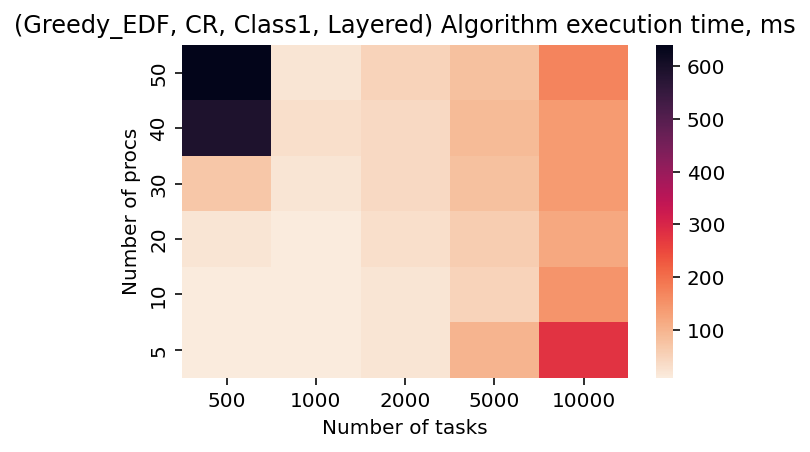
\includegraphics[width=\textwidth]{imgs/layered_class_1/CR_EDF/et_heatmap.png}
        \caption{Тепловая карта}
        \label{fig:CR-layered-EDF-exec-time-heatmap}
    \end{subfigure}
    \hfill
    \begin{subfigure}{0.49\textwidth}
        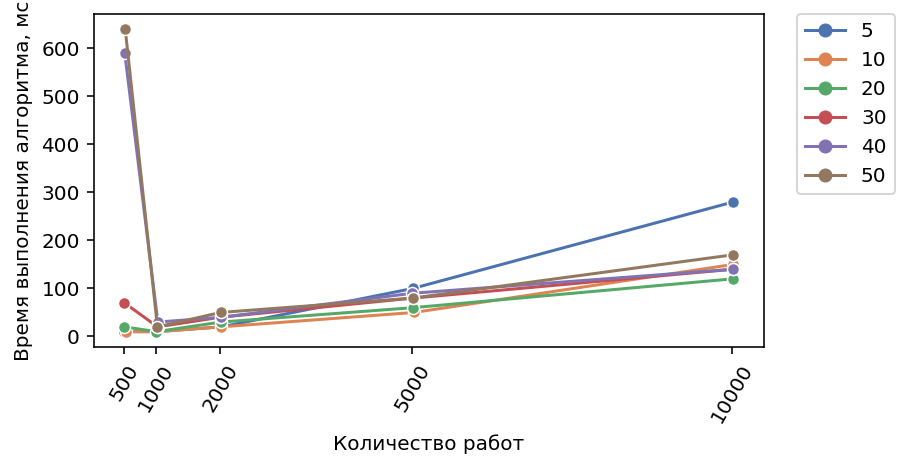
\includegraphics[width=\textwidth]{imgs/layered_class_1/CR_EDF/tr_graph.png}
        \caption{Сводный график}
        \label{fig:CR-layered-EDF-exec-time-compiled}
    \end{subfigure}
    \caption{Время выполнения алгоритма, в миллисекундах}
\end{figure}

На рисунках \ref{fig:CR-layered-EDF-exec-time-heatmap} и \ref{fig:CR-layered-EDF-exec-time-compiled} показано время выполнения жадного алгоритма с EDF эвристикой, включая прогоны METIS, на слоистых данных, основанных на слоистых графах. Как и для жадного алгоритма с жадной эвристикой, на данных видно два выброса, которые соотносятся с самым большим количеством процессором и самым маленьким количеством работ в исходных данных. Также не существует значимой зависимости между количеством процессоров в системе и временем, затраченным на построение расписания. Алгоритм работает в несколько раз быстрее жадного алгоритма.

\begin{figure}[!htbp]
    \centering
    \begin{subfigure}{0.49\textwidth}
        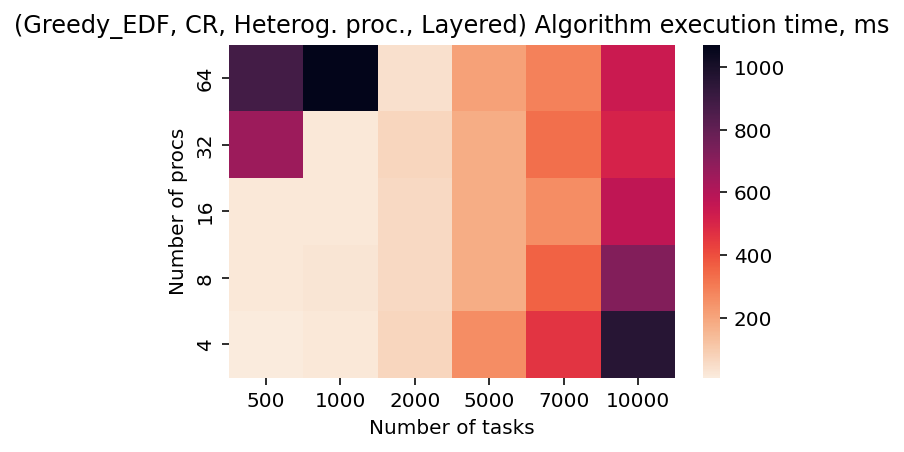
\includegraphics[width=\textwidth]{imgs/unbalanced/CR_EDF/et_heatmap.png}
        \caption{Тепловая карта}
        \label{fig:CR-unbalanced-EDF-exec-time-heatmap}
    \end{subfigure}
    \hfill
    \begin{subfigure}{0.49\textwidth}
        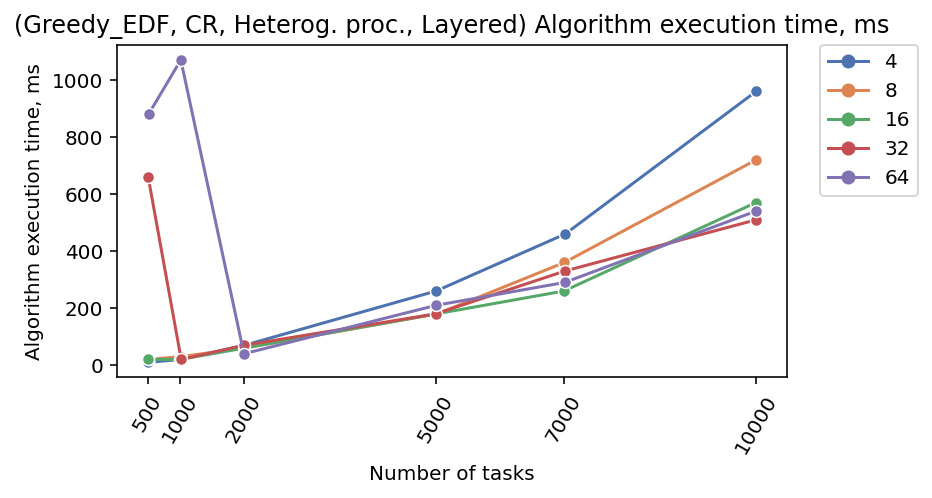
\includegraphics[width=\textwidth]{imgs/unbalanced/CR_EDF/tr_graph.png}
        \caption{Сводный график}
        \label{fig:CR-unbalanced-EDF-exec-time-compiled}
    \end{subfigure}
    \caption{Время выполнения алгоритма, в миллисекундах}
\end{figure}

На рисунках \ref{fig:CR-unbalanced-EDF-exec-time-heatmap} и \ref{fig:CR-unbalanced-EDF-exec-time-compiled} показано время выполнения жадного алгоритма с EDF эвристикой, включая прогоны METIS, на слоистых данных с неоднородными процессорами. Как и для жадного алгоритма с жадной эвристикой, на данных видно три выброса, которые соотносятся с самым большим количеством процессором и самым маленьким количеством работ в исходных данных. Также не существует значимой зависимости между количеством процессоров в системе и временем, затраченным на построение расписания. Алгоритм работает в несколько раз быстрее жадного алгоритма.

\paragraph{Постановка задачи без ограничений}

\begin{figure}[!htbp]
    \centering
    \begin{subfigure}{0.49\textwidth}
        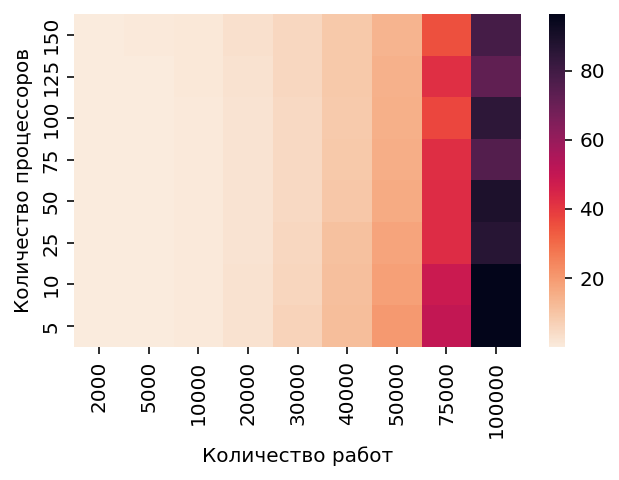
\includegraphics[width=\textwidth]{imgs/ideal_1/NO_EDF/et_heatmap.png}
        \caption{Тепловая карта}
        \label{fig:NO-EDF-exec-time-heatmap}
    \end{subfigure}
    \hfill
    \begin{subfigure}{0.49\textwidth}
        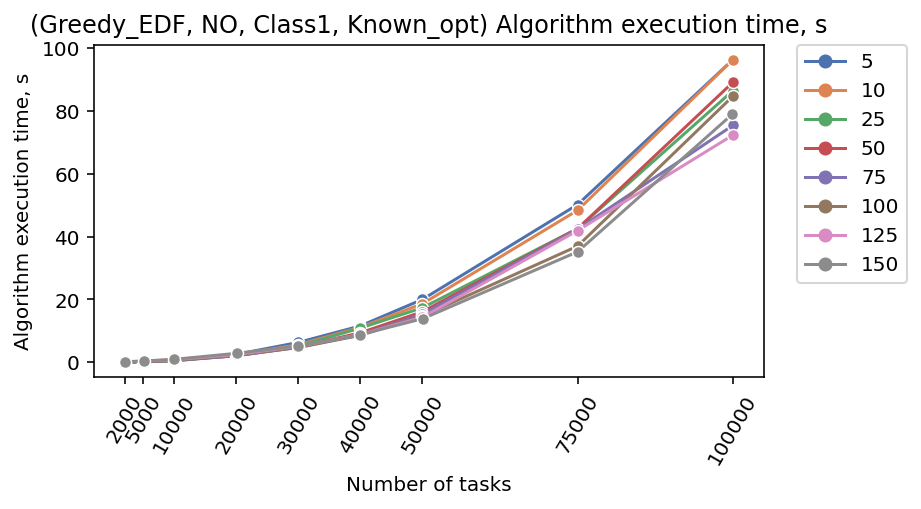
\includegraphics[width=\textwidth]{imgs/ideal_1/NO_EDF/tr_graph.png}
        \caption{Сводный график}
        \label{fig:NO-EDF-exec-time-compiled}
    \end{subfigure}
    \caption{Время выполнения алгоритма, в секундах}
\end{figure}

На рисунках \ref{fig:NO-EDF-exec-time-heatmap} и \ref{fig:NO-EDF-exec-time-compiled} показано время выполнения жадного алгоритма с EDF эвристикой, включая прогоны METIS, на данных с известным оптимумом.

\begin{figure}[!htbp]
    \centering
    \begin{subfigure}{0.49\textwidth}
        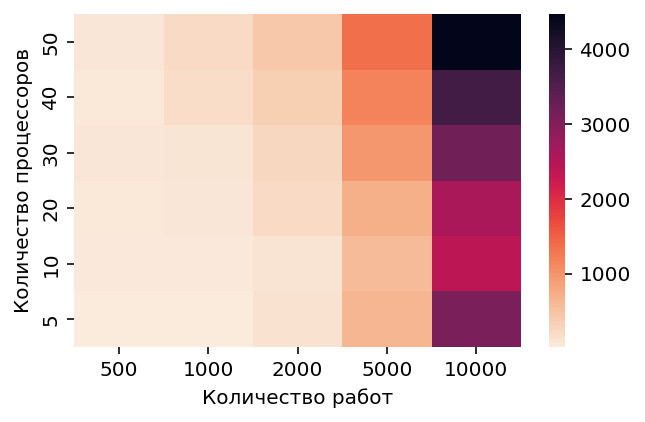
\includegraphics[width=\textwidth]{imgs/layered_class_1/NO_EDF/et_heatmap.png}
        \caption{Тепловая карта}
        \label{fig:NO-layered-EDF-exec-time-heatmap}
    \end{subfigure}
    \hfill
    \begin{subfigure}{0.49\textwidth}
        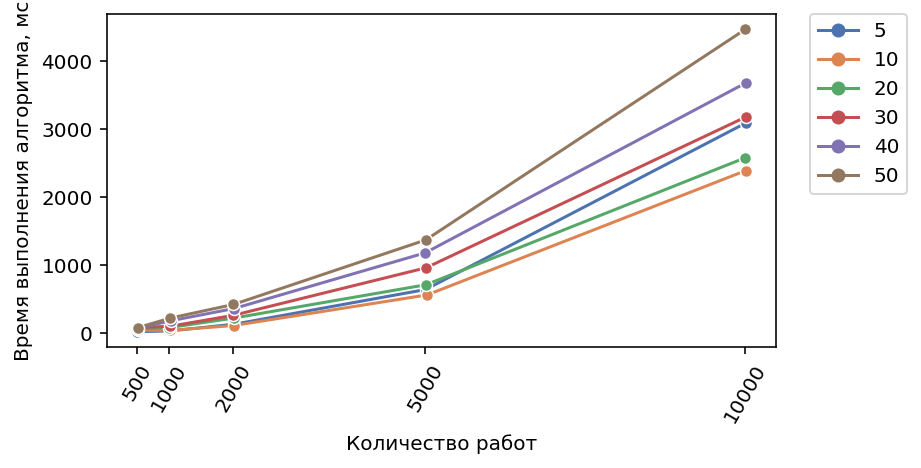
\includegraphics[width=\textwidth]{imgs/layered_class_1/NO_EDF/tr_graph.png}
        \caption{Сводный график}
        \label{fig:NO-layered-EDF-exec-time-compiled}
    \end{subfigure}
    \caption{Время выполнения алгоритма, в миллисекундах}
\end{figure}

На рисунках \ref{fig:NO-layered-EDF-exec-time-heatmap} и \ref{fig:NO-layered-EDF-exec-time-compiled} показано время выполнения жадного алгоритма с EDF эвристикой, включая прогоны METIS, на данных, основанных на слоистых графах.

\begin{figure}[!htbp]
    \centering
    \begin{subfigure}{0.49\textwidth}
        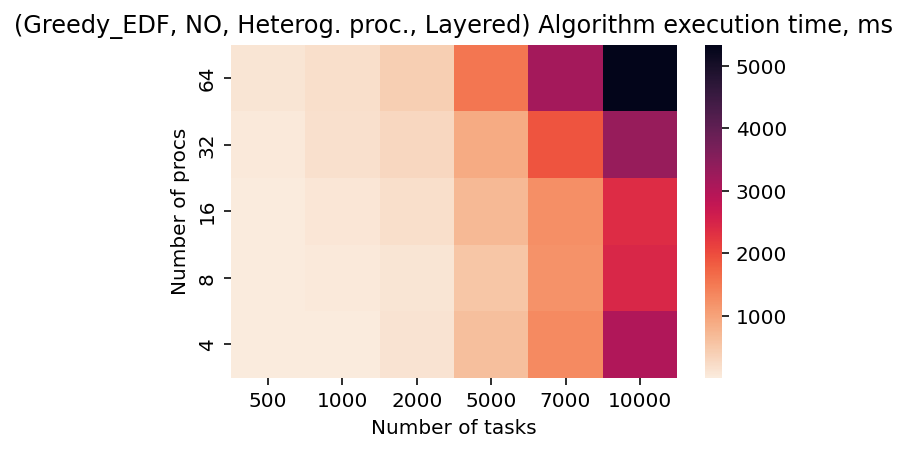
\includegraphics[width=\textwidth]{imgs/unbalanced/NO_EDF/et_heatmap.png}
        \caption{Тепловая карта}
        \label{fig:NO-unbalanced-EDF-exec-time-heatmap}
    \end{subfigure}
    \hfill
    \begin{subfigure}{0.49\textwidth}
        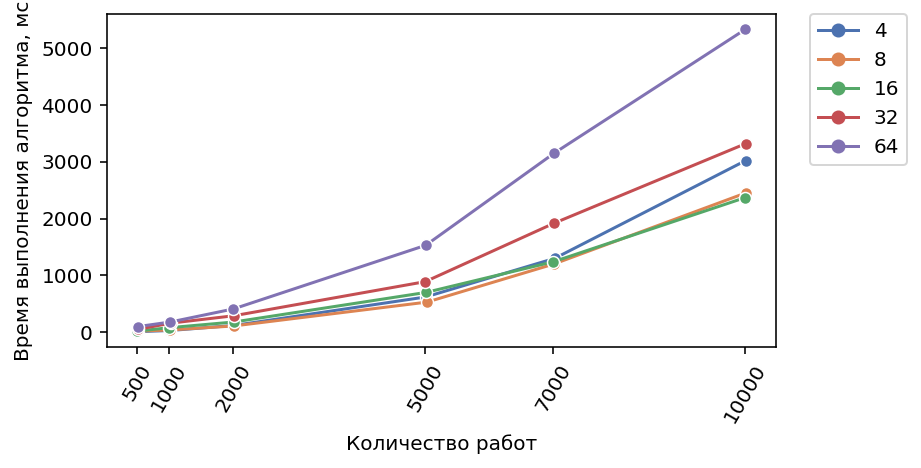
\includegraphics[width=\textwidth]{imgs/unbalanced/NO_EDF/tr_graph.png}
        \caption{Сводный график}
        \label{fig:NO-unbalanced-EDF-exec-time-compiled}
    \end{subfigure}
    \caption{Время выполнения алгоритма, в миллисекундах}
\end{figure}

На рисунках \ref{fig:NO-unbalanced-EDF-exec-time-heatmap} и \ref{fig:NO-unbalanced-EDF-exec-time-compiled} показано время выполнения жадного алгоритма с EDF эвристикой, включая прогоны METIS, на слоистых данных с неоднородными процессорами. Алгоритм выполняется быстрее жадного алгоритма, однако разница во времени выполнения незначительна. Время выполнения алгоритма увеличивается с увеличением количества работ и процессоров в системе.

\subsection{Выводы из экспериментального исследования}

% ----------------------------------------------------------------------------------------------------------------------
\newpage
\section{Заключение}
В ходе выполнения данной работы были достигнуты все ее цели, а именно:
\begin{enumerate}
    \item Проведен аналитический обзор алгоритмов построения списочных расписаний с целью выявления детерминированных алгоритмов, которые возможно модифицировать под поставленную задачу и имеют хорошую возможность масштабирования, по результатам которого были выбраны жадные алгоритмы.
    \item Разработаны и реализованы алгоритмы, основанные на различных жадных критериях.
    \item Проведено исследование свойств алгоритмов, которое показало низкую вычислительную сложность и среднее отклонение от оптимума в 30\% для жадного алгоритма с выбором по числу потомков и до 5-10\% для жадного алгоритма с фиктивными директивными сроками.
\end{enumerate}

При исследовании алгоритма были подобраны оптимальные параметры алгоритма и определены направления дальнейшего улучшения и исследования алгоритма.

% ----------------------------------------------------------------------------------------------------------------------
\newpage
\printbibliography

\appendix

% \newpage
% \intro{Классы входных данных}
% В данных, присланных от Хуавей существует разделение на 2 класса.
\begin{enumerate}
    \item Первый класс (примеры DAG\_A и DAG\_B) характеризуется относительно небольшим масштабом графа работ, небольшим числом процессоров, полнотой графа связности процессоров и одинаковыми задержками между любыми двумя процессорами.
    \item Второй класс (примеры DAG\_C и DAG\_D) характеризуется относительно большим масштабом графа работ, большим числом процессоров
\end{enumerate}
\begin{table}[!htbp]
    \begin{tabular}{c|c|c|c|c}
        & \multicolumn{4}{c}{Примеры входных данных}                            \\
        \hline
        Критерии            & DAG\_A                                     & DAG\_B & DAG\_C & DAG\_D \\
        \hline
        Масштаб графа работ & \makecell{45 вершин;                                                  \\75 ребер}                        & \makecell{1121 вершина;\\6229 ребер} & \makecell{197494 вершин;\\719389 ребер} & \makecell{1823309 вершин;\\6172920 ребер} \\
        \hline
        \makecell{Разброс                                                                           \\длительностей работ}            & 1-10                                       & 1-10   & \makecell{все работы\\одной длины} & \makecell{все работы\\одной длины} \\
        \hline
        \makecell{Связность                                                                         \\графа работ}                  & 1.66                                       & 5.55   & 3.64                   & 3.83                   \\
        \hline
        \makecell{Количество                                                                        \\процессоров}                 & 2                                          & 10     & 256                    & 4096                   \\
        \hline
        \makecell{Полный граф                                                                       \\связности\\процессоров}      & да                                         & да     & нет                    & да                     \\
        \hline
        \makecell{Одинаковые задержки                                                               \\на передачу данных} & да                                         & да     & да                     & нет                    \\
    \end{tabular}
    \caption{Сравнение примеров из классов данных}
\end{table}

\end{document}